%!TEX root = haiku.tex
\book{\LARGE \FK 日本近代五人俳句选}

\chapter[{\FM 正岡子規}]{\FM \ruby[g]{正}{まさ}\ruby[g]{岡}{おか}\ruby[g]{子}{し}\ruby[g]{規}{き}}

\begin{center}
    \begin{figure}
        \centering
        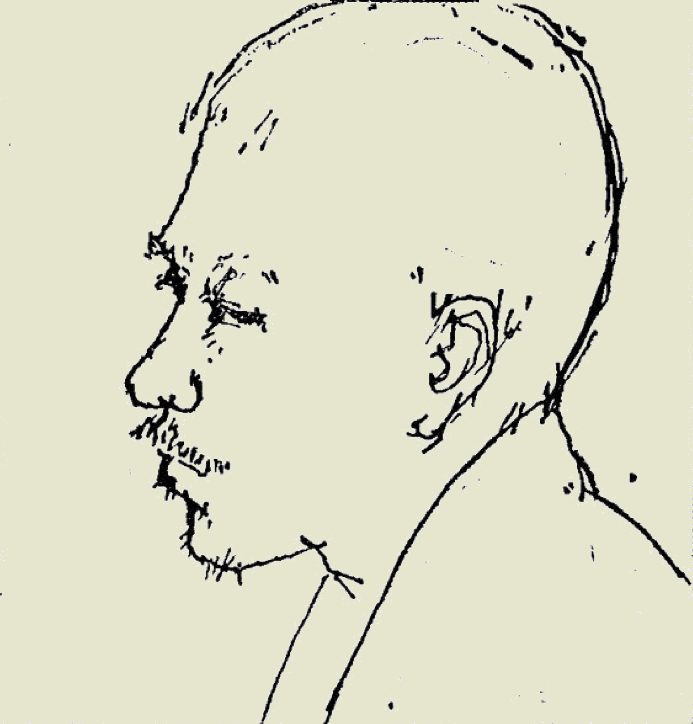
\includegraphics[height=0.9\textheight]{masaoka}\\[1em]
        \large{\FS 作~者~像}
    \end{figure}
\end{center}

\newpage
{\FS
    正冈子规(1867—1902),爱媛县松山市人,本名常规,别号獭祭书屋主人、竹子乡下人等。父隼太是松山藩士,母八重是著名汉学家大原观山之女。子规六岁丧父,由母亲抚养成人,年幼时跟外祖父大原观山和土屋文明学汉籍,奠定了深厚的汉学基础。十二岁写绝句《闻子规》:「一声孤月下,啼血不可闻,关夜空欹枕,故乡万里云。」显示出他的才华。一八八九年五月九日,二十三岁的子规开始咯血,是年取别号子规。他晚年长期卧病,但并不悲伤绝望,能乐观自处,在病床上写了动人的随笔《墨汁一滴》、《仰卧漫录》、《病床六尺》等。病情日渐恶化,逝世时才三十六岁。

    子规的一生虽然短暂,但他以坚韧不拔的努力,在明治时代文学史上留下了不可磨灭的功绩。他主张俳句和短歌应该革新,向江户末期的陈规陋习挑战,写了《獭祭屋俳话》、《俳句分类》、《俳谐大要》、《俳人芜村》等力作,在俳句创作上特别推崇芜村,使人们对芜村作品的艺术价值有了新的认识。

    子规作为俳人,可以说是一位承前启后的人物。他与芭蕉、芜村、一茶相比,因所处的时代、境遇和个人气质不同,俳风也就各异。子规主张「感情的文学,即纯粹的文学」,「美的标准,在于美的感情」。他的俳句,看来并非呕心沥血的苦吟,写景抒情,多为即兴之作。虽然他说过:「比起人事来,我更爱花鸟风月。」但晚年他也写了自以为较难写的人事写生句。可能是因为他在理论上过于强调写生,致使想象力不够丰富,生活又为病床所限,所以笔下的境界不够宽阔。他效法芜村的色彩美,也有汉诗的情调,俳风平易单纯,简洁明快,独树一帜。

    在短歌方面,他于一九〇二年发表《致歌人书》,又组织「根岸短歌会」,提倡短歌的革新,要求以写生法创作短歌,自己也效法《万叶集》的精神作了不少短歌,在歌坛有一定影响。

    附带说一下:我译的芭蕉、芜村、一茶的若干俳句发表以后,对我国友好的日本作家水上勉先生有一次对我说:「是否也译些正冈子规的俳句?」他这么一提,鼓起了我的勇气,我就开始阅读有关正冈子规的资料,并根据《子规全集》(共22卷,讲谈社1975年版)试译了俳句七十八首。译文也许未能传达原作的神韵,请读者指正。
}

\newpage

\section{\FK 新年}

\setcounter{haikucounter}{0}

\begin{haiku}
    {\FH \ruby[g]{初鶏}{はつとり}の、\ruby[g]{枕}{まくら}の上に、うたひける。}

    {\FK 正欲睡眠鸡报晓,岁序转新春。}
\end{haiku}

\begin{haiku}
    {\FH \ruby[g]{梅}{うめ}いけて、\ruby[g]{礼者}{れいしゃ}ことわる、\ruby[g]{病}{やまい}かな。}

    {\FK 瓶插梅花共贺春,谢客只因是病身。}
\end{haiku}

\begin{haiku}
    {\FH \ruby[g]{民}{たみ}の春、\ruby[g]{同胞}{どうほう}三千、九百万。}

    {\FK 同胞三千九百万,共庆过新年。}
\end{haiku}

\section{\FK 春}

\setcounter{haikucounter}{0}

\begin{haiku}
    {\FH 春の山、\ruby[g]{焼}{や}いたあとから、\ruby[g]{笑}{わら}ひけり。}

    {\FK 春山烧后露笑容。}
\end{haiku}

\begin{haiku}
    {\FH あたゝかな、雨がふるなり、\ruby[g]{枯葎}{かれむぐら}。}

    {\FK 温雨纷纷下,蔓草枯干不见芽。}

    {\FT 注:温雨即初春的雨,有暖意。}
\end{haiku}

\begin{haiku}
    {\FH 春雨や、\ruby[g]{唐撫子}{からなでしこ}の、死を\ruby[g]{惜}{おし}む。}

    {\FK 春雨霏霏,哀哉石竹凋萎!\footnote{\FT 此句实为高滨虚子所作。}}
\end{haiku}

\begin{haiku}
    {\FH \ruby[g]{陽炎}{かげろう}や、日本の土に、\ruby[g]{殯}{かりもがり}。}

    {\FK 游丝呀,埋葬东瀛泥土下!}

    {\FT 注:以上两句是哀悼子规的中国弟子苏山人之作。苏山人(1881—1902)姓罗名朝斌,字卧云,号听松,江苏苏州人,父罗庚龄为清朝驻日公使何如璋的译员,母是日本人。苏山人自幼喜爱文学诗歌,后拜正冈子规为师,交游颇广。他的俳句被收在子规编辑的《春夏秋冬》、《明治俳句》专集中。一九〇二年春因病在东京逝世,年仅二十二岁。}
\end{haiku}

\begin{haiku}
    {\FH 島々に、\ruby[g]{灯}{ひ}をともしけり、春の海}

    {\FK 岛岛点起了灯火,春之海啊。}
\end{haiku}

\begin{haiku}
    {\FH \ruby[g]{一桶}{いちおけ}の、\ruby[g]{藍}{あい}\ruby[g]{流}{なが}しけり、春の川。}

    {\FK 春日河川上,正是一桶靛蓝流。}

    {\FT 注:这是子规流畅体。作者把春天河川的水比作一桶流动的蓝颜料,这景象在乡下有染坊的地方可以看到。\footnote{\FT 此句出自《病床六尺》,据子规自注,确实是一桶随波飘荡的蓝色颜料,而不是形容河水被染成蓝色。}}
\end{haiku}

\begin{haiku}
    {\FH 春風に、\ruby[g]{零}{こぼれ}て赤し、\ruby[g]{歯}{はみ}\ruby[g]{磨}{がき}\ruby[g]{粉}{こ}。}

    {\FK 洒落春风牙粉红。}

    {\FT 注:子规早晨刷牙时因咯血而染红了牙粉。此句用红白的色彩感来描写病状,没有悲伤意。}
\end{haiku}

\begin{haiku}
    {\FH 春の日や、\ruby[g]{病床}{びょうしょう}にして、絵の\ruby[g]{稽古}{けいこ}。}

    {\FK 春日病床上,学画来消遣。}

    {\FT 注:子规喜画,但无老师,只把花果放在床边,随笔写生。}
\end{haiku}

\begin{haiku}
    {\FH とろとろと、\ruby[g]{左官}{さかん}眠るや、\ruby[g]{燕}{つばくらめ}。}

    {\FK 泥工打瞌睡,燕子正交飞。}

    {\FT 注:此句写农村的泥工盖新房午休时的情景。}
\end{haiku}

\begin{haiku}
    {\FH ひらひらと、風に流れて、\ruby[g]{蝶}{ちょう}一つ。}

    {\FK 蝴蝶翩翩飞去,风吹又飞回。}
\end{haiku}

\begin{haiku}
    {\FH \ruby[g]{茨}{いばら}にかけし、\ruby[g]{胡蝶}{こちょう}の羽の、\ruby[g]{破}{やぶ}れたる。}

    {\FK 蝴蝶碰荆棘,刺破了翅膀。}

    {\FT 注:美丽的翅膀受了损伤,令人惋惜。}
\end{haiku}

\begin{haiku}
    {\FH \ruby[g]{白魚}{しらうお}や、\ruby[g]{椀}{わん}の中にも、角田川。}

    {\FK 银鱼碗里鲜,联想角田川。}

    {\FT 注:银鱼在日语中叫白鱼,角田川现称隅田川。}
\end{haiku}

\begin{haiku}
    {\FH \ruby[g]{若鮎}{わかあゆ}の、二手になりて、\ruby[g]{上}{のぼ}りけり。}

    {\FK 石手川出合渡}

    {\FK 小香鱼,分两路溯流游去。}

    {\FT 注:石手川出合渡是松山市内的重信川与郊外的石手川合流的渡口,活泼的小香鱼在合流处分二路溯流而上。}
\end{haiku}

\begin{haiku}
    {\FH 茶屋もなく、\ruby[g]{酒屋}{さかや}も見えず、花一木。}

    {\FK 茶楼酒馆无踪迹,唯见娇艳花一枝。}
\end{haiku}

\begin{haiku}
    {\FH 桃梅を、笑へば梅も、桃を笑らふ。}

    {\FK 国会开幕}

    {\FK 桃嘲梅来梅笑桃。}
\end{haiku}

\begin{haiku}
    {\FH 人載せて、牛載せて桃の、渡し哉。}

    {\FK 载人又载牛,喧闹桃渡口。}
\end{haiku}

\begin{haiku}
    {\FH 紅梅の、散りぬ\ruby[g]{淋}{さび}しき、枕元。}

    {\FK 红梅花散落,寂寞枕头边。}
\end{haiku}

\begin{haiku}
    {\FH 夢に美人、来れり\ruby[g]{曰}{いわ}く、梅の精と。}

    {\FK 梦里美人来,说是梅花精。}

    {\FT 注:这是妖艳句,颇有芜村的风格。}
\end{haiku}

\begin{haiku}
    {\FH 僧や俗や、梅活けて\ruby[g]{発句}{はっく}、十五人。}

    {\FK 松山松风会席上}

    {\FK 花瓶插红梅,僧俗俳句十五人。}
\end{haiku}

\begin{haiku}
    {\FH \ruby[g]{鞦韆}{しゅうせん}の、影静かなり、梨花の月。}

    {\FK 秋千影静静,梨花月有阴。}

    {\FT 注:此句意境与苏轼《春宵》中的「花有清香月有阴……秋千院落夜沉沉」略同。}
\end{haiku}

\begin{haiku}
    {\FH 一つ落ちて、二つ落ちたる、\ruby[g]{椿}{つばき}哉。}

    {\FK 山茶花啊,落了一朵,落了两朵。}

    {\FT 注:这三句略似小幅写生画,给人留下鲜明印象,句中有时间的推移,使人仿佛目睹艳丽的景物。}
\end{haiku}

\begin{haiku}
    {\FH 山吹の、雨やガラスの、窓の外。}

    {\FK 玻璃窗外,棠棣花雨飘。}
\end{haiku}

\section{\FK 夏}

\setcounter{haikucounter}{0}

\begin{haiku}
    {\FH 夏嵐、\ruby[g]{机上}{きじょう}の\ruby[g]{白紙}{はくし}、飛び\ruby[g]{尽}{つく}す。}

    {\FK 夏日山风来,桌上白纸尽飞去。}
\end{haiku}

\begin{haiku}
    {\FH 五月雨や、\ruby[g]{けふ}{きょう}も上野を、見てくらす。}

    {\FK 梅雨时节,看厌上野山色。}
\end{haiku}

\begin{haiku}
    {\FH \ruby[g]{陣笠}{じんがさ}を、着た人もある、\ruby[g]{田植}{たうえ}哉。}

    {\FK 插秧农田里,还有戴盔人。}

    {\FT 注:藩士退役归田,从事农耕,插秧时还戴着战盔。此句表示时代已变化,仍留旧迹象。}
\end{haiku}

\begin{haiku}
    {\FH 暁や、白帆過ぎ行く、\ruby[g]{蚊帳}{かや}の外。}

    {\FK 拂晓时分,白帆驶过蚊帐外。}

    {\FT 注:子规在海边须磨疗养院的卧室里,晨曦照在绿色的蚊帐上,此时他意外地看见白帆在海上驶过。}
\end{haiku}

\begin{haiku}
    {\FH \ruby[g]{柳}{やなぎ}伐って、\ruby[g]{翡翠}{かわせみ}\ruby[g]{遂}{つい}に、来ずなりぬ。}

    {\FK 柳树被伐采,终于不见翡翠来。}

    {\FT 注:子规认为梅与莺、竹与雀、杨柳与翡翠的配合,虽是陈旧的程式,但也有其美感。翡翠总是站在水边的柳枝上想啄食水中的游鱼,柳树既被砍掉,翡翠失去立脚点,就到别处去了。}
\end{haiku}

\begin{haiku}
    {\FH \ruby[g]{看}{かん}\ruby[g]{護}{ご}\ruby[g]{婦}{ふ}や、うたゝ寝さめて、\ruby[g]{蝿}{はえ}を打つ。}

    {\FK 看护妇打瞌睡,醒来拍苍蝇。}

    {\FT 注:伺候子规的看护妇瞌睡醒后,不好意思,拿蝇拍打苍蝇,这写出了一种心理状态。}
\end{haiku}

\begin{haiku}
    {\FH 林檎くふて、牡丹の前に、死なん哉。}

    {\FK 饱啖苹果后,死在牡丹前。}

    {\FT 注:一八九六年五月十七日,子规从中国归国的途中,在船上咯血,二十八日进入神户病院。翌年四月五日做了两次手术。一八九九年五月,子规发烧、失眠、腰痛,食欲不振,病势较重,因不堪其苦,故吟此辞世句。}
\end{haiku}

\begin{haiku}
    {\FH \ruby[g]{銀屏}{ぎんびょう}や、\ruby[g]{崩}{くず}れんとする、白牡丹。}

    {\FK 华丽银屏前,烂漫将谢白牡丹。}

    {\FT 注:银屏配白牡丹,那是满屋生辉的景色,但此句只写白牡丹盛开将谢的状态。这是艳丽句体。}
\end{haiku}

\begin{haiku}
    {\FH 土\ruby[g]{一塊}{いっかい}、牡丹いけたる、其下に。}

    {\FK 自题}

    {\FK 牡丹花瓶下,泥土一块。}

    {\FT 注:一九〇二年五月,子规为病情所苦而作此句,题在香取秀真为他塑制的石膏像背面。作者认为自己死之将至,犹如艳丽的牡丹花下的一块泥土。}
\end{haiku}

\begin{haiku}
    {\FH 赤き薔薇、白き薔薇皆、さみだるゝ。}

    {\FK 红蔷薇,白蔷薇,湿润梅雨水。}
\end{haiku}

\begin{haiku}
    {\FH 薔薇を剪る、\ruby[g]{鋏刀}{はさみ}の音や、\ruby[g]{五月}{さつき}\ruby[g]{晴}{ばれ}。}

    {\FK 听得蔷薇剪刀声,正是五月梅雨晴。}
\end{haiku}

\begin{haiku}
    {\FH 朝顔や、紫しぼる、朝の雨。}

    {\FK 牵牛花色艳,染得晨雨亦紫妍。}

    {\FT 注:晨雨接触牵牛花,染上紫艳颜色,染字成为句的主眼,上下全活了。}
\end{haiku}

\begin{haiku}
    {\FH \ruby[g]{蕣}{あさがお}や、君いかめしき、文学士。}

    {\FK 牵牛正值开花时,迎接堂堂文学士。}

    {\FT 注:夏目漱石对文部省授给文学博士的称名,十分讨厌,曾坚决谢绝,但谢绝不了。子规在此句中,用「堂堂」二字,有点打趣。}
\end{haiku}

\begin{haiku}
    {\FH 青梅や、黄梅やうつる、\ruby[g]{軒}{のき}らんぷ。}

    {\FK 檐下油灯明,青梅黄梅相照映。}

    {\FT 注:梅雨季节,梅子未熟的叫青梅,熟的叫黄梅。}
\end{haiku}

\begin{haiku}
    {\FH 若竹や、四五本青き、庭の\ruby[g]{隅}{すみ}。}

    {\FK 一角庭院边,嫩竹青青四五竿。}
\end{haiku}

\begin{haiku}
    {\FH 舟行くや、\ruby[g]{小鬢}{こびん}にさはる、\ruby[g]{蓮}{はす}の花。}

    {\FK 舟行在莲塘,莲花碰触小鬓上。}

    {\FT 注:梁武帝有五言诗:「采莲南塘秋,莲花过人头。」子规把「过」改为「碰」,都是美丽的画面。}
\end{haiku}

\section{\FK 秋}

\setcounter{haikucounter}{0}

\begin{haiku}
    {\FH 天の川、こぼれ落ちたる、星一つ。}

    {\FK 夜凉如水,银河岸畔,星一颗。}
\end{haiku}

\begin{haiku}
    {\FH \ruby[g]{門}{かど}を出て、十歩に秋の、海廣し。}

    {\FK 出门走十步,秋日海天阔。}
\end{haiku}

\begin{haiku}
    {\FH 旅の旅、又その旅の、秋の風。}

    {\FK 旅行又旅行,秋风尽在旅途中。}

    {\FT 注:这是一八九二年所作的俳句,写他在十月间无休止的旅行,又在旅途中感到秋风的寒意,同时也反映他是在人生的道路上。}
\end{haiku}

\begin{haiku}
    {\FH 秋の山、\ruby[g]{御幸寺}{みゆきじ}と申し、天狗住む。}

    {\FK 秋山御幸寺,天狗住其中。}

    {\FT 注:山在松山北郊,人们叫它作御幸寺。山形怪异,相传有天狗在那里,令人恐惧。天狗是想象中的怪物,住在深山中,状如人,红脸高鼻,有翅膀,飞行自如。}
\end{haiku}

\begin{haiku}
    {\FH 長き夜や、孔明死する、三國志。}

    {\FK 长夜览读《三国志》,正到孔明病殁时。}
\end{haiku}

\begin{haiku}
    {\FH 長き夜の、面白きかな、\ruby[g]{水滸傳}{すいこでん}。}

    {\FK 阅读《水浒传》,夜长妙趣多。}

    {\FT 注:子规自少年时代,便爱读军事历史小说之类,《水浒传》、《三国演义》也是他爱读的书。}
\end{haiku}

\begin{haiku}
    {\FH 長き夜や、人灯を取って、庭に行く。}

    {\FK 人提灯火穿院去,夜里依然又静寂。}

    {\FT 注:写静中有动,动后仍归于静,这是着重于听觉的句子。}
\end{haiku}

\begin{haiku}
    {\FH 行く我に、とどまる\ruby[g]{汝}{なれ}に、秋二つ。}

    {\FK 别漱石}

    {\FK 我去你留,两个秋。}

    {\FT 注:子规从松山要去东京,夏目漱石仍旧逗留松山。两人分别,时在秋天,惜别又叹境遇不同,巧妙地用了两个秋。}
\end{haiku}

\begin{haiku}
    {\FH \ruby[g]{芋}{いも}の\ruby[g]{用意}{ようい}、酒の用意や、人遲し。}

    {\FK 煮芋又备酒,宾客何来迟。}

    {\FT 注:一八九七年八月十七日,在上野元光院赏月,又听筑前琵琶。到会者约二十人。此句写月出前的准备工作。}
\end{haiku}

\begin{haiku}
    {\FH あるが中に、\ruby[g]{詩人}{しじん}\ruby[g]{痩}{や}せたり、月の宴。}

    {\FK 赏月雅会里,诗人貌清瘦。}

    {\FT 注:雅会中的诗人,指汉诗人本田种竹山人之辈,子规和他交往,谈论汉诗,曾有汉诗《访种竹君听诗话而还》。}
\end{haiku}

\begin{haiku}
    {\FH ある僧の、月も待たずに、歸りけり。}

    {\FK 旧历八月十七日元光院}

    {\FK 不待明月出,有僧竟自归。}

    {\FT 注:一八九八年相约于中秋后两天赏「立待月」,子规也稍微迟到参加了。但其中释清潭不知何故却早离席。高滨虚子以为此句有弦外之音,说此僧人胸无点墨,不能强为吟咏,故早退席。}
\end{haiku}

\begin{haiku}
    {\FH \ruby[g]{病床}{びょうしょう}の、\ruby[g]{呻}{うめ}きに\ruby[g]{和}{なご}して、秋の蝉。}

    {\FK 病床苦呻吟,秋蝉来唱和。}

    {\FT 注:到了秋天,蝉断断续续衰弱的叫声,跟病者的呻吟声,有点合调。}
\end{haiku}

\begin{haiku}
    {\FH \ruby[g]{木犀}{もくせい}や、母が\ruby[g]{教}{をし}ふる、\ruby[g]{二絃琴}{にげんきん}。}

    {\FK 木樨花正发,母教二弦琴。}
\end{haiku}

\begin{haiku}
    {\FH 月\ruby[g]{落}{おち}て、\ruby[g]{江村}{こうそん}\ruby[g]{蘆}{あし}の、花白し。}

    {\FK 江村月夜芦花白。}
\end{haiku}

\begin{haiku}
    {\FH \ruby[g]{骨}{こ}も見えず、むくろも見えず、草の花。}

    {\FK 吊古战场}

    {\FK 尸骨皆不见,唯有草花妍。}
\end{haiku}

\begin{haiku}
    {\FH \ruby[g]{柿}{かき}食へば、\ruby[g]{鐘}{かね}が鳴るなり、\ruby[g]{法隆寺}{ほうりゅうじ}。}

    {\FK 在法隆寺茶店小憩}

    {\FK 我尝柿子时,钟鸣法隆寺。}

    {\FT 注:吃柿子时听到钟声,两者虽无关联,只因为是同时发生的事,就把它们联系起来。}
\end{haiku}

\begin{haiku}
    {\FH 三千の、俳句を\ruby[g]{閲}{けみ}し、柿二つ。}

    {\FK 俳句检阅三千首,枕边柿子两个。}

    {\FT 注:子规在《日本》报刊上创设俳句栏,是他的革新事业的中心。有一天要夜以继日地看来稿俳句三千首,从中选用,工作颇为繁忙。枕边放着爱吃的两个柿子。「两个」和「三千」是数字的照应。}
\end{haiku}

\begin{haiku}
    {\FH 冬近き、嵐に折れし、\ruby[g]{鷄頭}{けいとう}哉。}

    {\FK 幼嫩鸡冠花,那堪飙风刮?}

    {\FT 注:子规酷爱鸡冠花,以拟人法描写它。}
\end{haiku}

\begin{haiku}
    {\FH 鷄頭の、十本ばかり、百姓家。}

    {\FK 寻常百姓家,将开十蕊鸡冠花。}
\end{haiku}

\begin{haiku}
    {\FH \ruby[g]{案山子}{かかし}物、言て\ruby[g]{猶}{なお}淋しぞ、秋の\ruby[g]{暮}{くれ}。}

    {\FK 稻草人也感寂寞,当此秋之暮。}
\end{haiku}

\begin{haiku}
    {\FH 柳散り、菜\ruby[g]{屑}{くず}流るゝ、小川哉。}

    {\FK 根岸音无川}

    {\FK 柳叶已凋萎,菜屑小川漂。}

    {\FT 注:根岸与日暮里之间有条小川,名叫音无川。秋冬时附近居民在这小川洗净蔬菜。}
\end{haiku}

\begin{haiku}
    {\FH \ruby[g]{白萩}{しろはぎ}の、しきりに露を、こぼしけり。}

    {\FK 风吹白色胡枝子,花露点点滴。}

    {\FT 注:这是写秋天庭院的美,秋风吹拂白萩花露滴落的情景。}
\end{haiku}

\begin{haiku}
    {\FH 驚くや、夕顔落ちし、\ruby[g]{夜半}{よわ}の音。}

    {\FK 夜半惊醒梦,瓠瓜落地声。}

    {\FT 注:某夜深时,有一种声音,使子规从梦中惊醒过来,后来才知道是院子的瓠瓜棚上结的瓠瓜落地的声音。声音微小,子规也这么震动,可见他的身体衰弱。}
\end{haiku}

\begin{haiku}
    {\FH 草花を、畫く日課や、秋に入る。}

    {\FK 入秋时节,绘草描花作日课。}

    {\FT 注:子规好作画,入秋画画,聊以自慰,将盆裁的草花摆到枕边作写生之用。据云最初画的草花是秋海棠。此句是他的生活写照。}
\end{haiku}

\begin{haiku}
    {\FH \ruby[g]{糸瓜}{へちま}\ruby[g]{咲}{さい}て、\ruby[g]{痰}{たん}のつまりし、仏かな。}

    {\FK 丝瓜放蕊时,痰塞成佛去。}
\end{haiku}

\begin{haiku}
    {\FH 痰一斗、糸瓜の水も、間にあはず。}

    {\FK 良药丝瓜水,难治一斗痰。}
\end{haiku}

\begin{haiku}
    {\FH をととひの、糸瓜の水も、取らざりき。}

    {\FK 前日丝瓜水,不曾饮入嘴。}

    {\FT 注:丝瓜是止咳消痰的药材,曾在自己的院子做棚种植\footnote{{\FT 前文有述子规的院子里有瓠瓜棚,瓠瓜和丝瓜不是同一种植物。丝瓜的学名} \emph{Lagenaria siceraria} var. \emph{hispida} {\FT ,和瓠瓜同属葫芦科。}},入药用。}

    {\FT 以上是绝笔的三首俳句。子规的病况,一九〇二年九月十日起,两腿浮肿,一点也不能动弹,但精神却很平稳,意识到死神已经迫近,终于在十九日午前一时逝世。}
\end{haiku}

\section{\FK 冬}

\setcounter{haikucounter}{0}

\begin{haiku}
    {\FH \ruby[g]{小夜}{さよ}\ruby[g]{時雨}{しぐれ}、上野を虚子の、來つゝあらん。}

    {\FK 病中}

    {\FK 夜半时雨降,虚子可从上野来?}

    {\FT 注:子规殷切希望弟子高滨虚子早一点来。}
\end{haiku}

\begin{haiku}
    {\FH いくたびも、雪の深さを、\ruby[g]{尋}{たず}ねけり。}

    {\FK 病中雪}

    {\FK 频频寻问,积雪深几许?}

    {\FT 注:久卧病床的子规,总想接触外界,问了妹妹,又问妈妈,使她们不得不跑出门外看雪,再回答子规。这句写出子规难以抑制挂念积雪的心情,是他的代表作之一。}
\end{haiku}

\begin{haiku}
    {\FH 冬\ruby[g]{籠}{こもり}、日記に梦を、書きつける。}

    {\FK 目记存梦境,闭门严冬静。}
\end{haiku}

\begin{haiku}
    {\FH 雪の跡、木履\ruby[g]{草鞋}{わらじ}の、別れかな。}

    {\FK 雪中送客去,留下草鞋木屐痕。}
\end{haiku}

\begin{haiku}
    {\FH 冬\ruby[g]{枯}{がれ}や、巡査に\ruby[g]{吠}{ほ}える、里の犬。}

    {\FK 荒寒少客行,村犬吠巡警。}
\end{haiku}

\begin{haiku}
    {\FH \ruby[g]{鷹狩}{たかがり}や、豫陽の太守、武を\ruby[g]{好}{この}む。}

    {\FK 尚武豫阳太守,放鹰猎获野兽。}
\end{haiku}

\begin{haiku}
    {\FH しぐるゝや、むれて押しあふ、桶の\ruby[g]{鮒}{ふな}。}

    {\FK 鲫鱼惊阵雨,竞相逃避一桶里。}

    {\FT 注:屋外桶里的鲫鱼,因阵雨滴落,在狭窄的桶里竞相逃避,这是写小景、近景的俳句。}
\end{haiku}

\begin{haiku}
    {\FH \ruby[g]{暖爐}{だんろ}\ruby[g]{焚}{た}くや、\ruby[g]{玻璃}{はり}窓外の、風の松。}

    {\FK 室中炉火盛,玻璃窗外松涛声。}
\end{haiku}

\begin{haiku}
    {\FH 水仙も、處を得たり、庭の隅。}

    {\FK 贺新居}

    {\FK 水仙得其所,庭隅自不俗。}
\end{haiku}

\begin{haiku}
    {\FH 梅活けて、君待つ\ruby[g]{庵}{いお}や、\ruby[g]{大}{おお}\ruby[g]{三十}{みそ}\ruby[g]{日}{か}。}

    {\FK 漱石约来寓}

    {\FK 时逢除夕岁将尽,插就梅花等待君。}
\end{haiku}

\chapter[{\FM 夏目漱石}]{\FM \ruby[g]{夏}{なつ}\ruby[g]{目}{め}\ruby[g]{漱}{そう}\ruby[g]{石}{せき}}

\begin{center}
    \begin{figure}
        \centering
        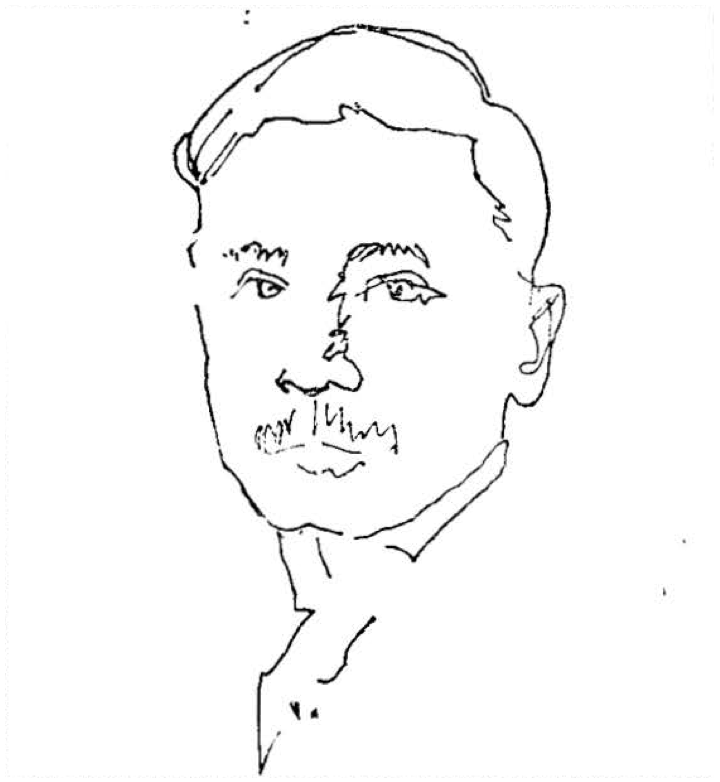
\includegraphics[height=0.9\textheight]{natsume}\\[1em]
        \large{\FS 作~者~像}
    \end{figure}
\end{center}

\newpage

{\FS
    夏目漱石(1867—1916)生于江户牛込马场下横町的一个小官吏的家庭,本名金之助。一八九三年东京帝国大学英文科毕业后,先后在东京专门学校、东京高等师范学校、爱媛县松山中学教英文。一九〇〇年被文部省派往英国伦敦留学,研究英国文学。留学期间,备受冷落,极不愉快。回国后对当时社会非常愤懑。一九〇五年在《杜鸥》杂志上发表《我是猫》(长篇讽刺小说),一九〇六年发表小说《哥儿》,批判教育界不良现象,于是声名大振,同年发表俳句情趣的小说《旅宿》,主人公是一个画家,避开讨厌的世俗,外出旅行,寻求澄清心境的桃源。一九〇七年他辞去教职,任《朝日新闻》文艺栏主编,在该报发表三部曲《三四郎》、《其后》和《门》,反映了知识分子在黑暗社会寻求出路的窘状。他遂成为日本杰出的批判现实主义作家。

    夏目漱石在思想上受了儒学与禅宗的影响。在创作风格上属于「余裕派」,主张以旁观者的立场和悠然自得的态度,吟咏自然、艺术和人生。他特别赏识「读万卷书而为万里游」的名言,一位日本评论家说:「其文雄俊博大,卓然有奇气。」

    夏目漱石少年时代从东京第一中学转入二松学舍学习汉学,并练习写作,也曾想以汉学立身。晚年写很多汉诗,对于格律、平仄、押韵和对仗运用自如。诗虽多无题,而情味甚浓,兹请读其临终前二旬间写的一首七律:
    \begin{center}
        真踪寂寞杳难寻,欲抱虚怀步古今。

        碧水碧山何有我,盖天盖地是无心。

        依稀暮色月离草,错落秋声风在林。

        眼耳双忘身亦失,空中独唱白云吟。
    \end{center}

    他很早就写俳句,一八九五年在松山中学任教时,与正冈子规同住过愚陀佛庵公寓,过从甚密,参加过子规指导的松风会活动。一生所写的俳句约达二四五〇首。在松山写的俳句占三分之一,并用过愚陀佛的笔名。他和子规是同龄人,曾受子规的影响,尊重子规所倡导的写实,但也发展自己浪漫气氛与洒脱畅达的特色。子规曾赞其俳句「雄键,无往而不雄健;真诚,无往而不真诚」。夏目漱石写作俳句的热情后来减退,专事小说创作。一九一五年开始在《朝日新闻》上连载长篇小说《明暗》,但还没写完就因病逝世,终年五十岁。本集中所选四十六首俳句,都是根据《夏目漱石全集》第二十三卷(岩波书店1984年版)翻译的。
}

\newpage

\section{\FK 新年}

\setcounter{haikucounter}{0}

\begin{haiku}
    {\FH \ruby[g]{五斗米}{ごとべい}を、\ruby[g]{餅}{もち}にして喰ふ、春来たり。}

    {\FK 新春已来到,五斗米做饼吃。}
\end{haiku}

\begin{haiku}
    {\FH \ruby[g]{金泥}{きんでい}の、鶴や\ruby[g]{朱塗}{しゅぬり}の、\ruby[g]{屠蘇}{とそ}の\ruby[g]{盆}{ぼに}。}

    {\FK 泥金仙鹤画,涂朱屠苏杯。}
\end{haiku}

\begin{haiku}
    {\FH 温泉や、水\ruby[g]{滑}{なめ}らかに、去年の\ruby[g]{垢}{あか}。}

    {\FK 温泉水滑,洗去旧年油垢。}

    {\FT 注:「温泉水滑」取自白居易《长恨歌》中的「温泉水滑洗凝脂」。}
\end{haiku}

\begin{haiku}
    {\FH \ruby[g]{光琳}{こうりん}の、\ruby[g]{屏風}{びょうぶ}に咲くや、\ruby[g]{福寿草}{ふくじゅそう}。}

    {\FK 福寿草花,开在光琳屏风上。}

    {\FT 注:福寿草即侧金盏花,黄色多瓣,增添新春气氛。光琳即尾形光琳(1658—1716),日本名画家。}
\end{haiku}

\section{\FK 春}

\setcounter{haikucounter}{0}

\begin{haiku}
    {\FH \ruby[g]{馬子唄}{まごうた}や、\ruby[g]{白髪}{しらが}も染めで、暮るゝ春。}

    {\FK 马夫歌声处,白发对暮春。}

    {\FT 注:小说《旅宿》载此句,指山村老太婆难耐凄凉,几经岁月数着过路的马。}
\end{haiku}

\begin{haiku}
    {\FH 春風や、\ruby[g]{惟然}{いぜん}が耳に、馬の鈴。}

    {\FK 惟然耳边声,春风吹马铃。}

    {\FT 注:广漱惟然是江户时代前期俳人芭蕉的门人。句写登山之后,景象寂寥。似以惟然自况。}
\end{haiku}

\begin{haiku}
    {\FH 春寒し、\ruby[g]{墓}{はか}に\ruby[g]{懸}{か}けたる、季子の剣。}

    {\FK 春寒暮树,挂着季子的剑。}

    {\FT 注:春秋吴国季札给逝世的徐君赠剑的故事。}
\end{haiku}

\begin{haiku}
    {\FH 人に死し、鶴に生れて、\ruby[g]{冴返}{さえかえ}る。}

    {\FK 人死转生鹤,高洁又清和。}

    {\FT 注:有的评论家认为此作富于浪漫主义幻想,有着离俗的格调,是个几乎难以企及的秀句。}
\end{haiku}

\begin{haiku}
    {\FH \ruby[g]{腸}{はらわた}に、春\ruby[g]{滴}{したた}るや、\ruby[g]{粥}{かゆ}の味。}

    {\FK 粥味滴滴香,春入肠胃。}

    {\FT 注:作者患胃溃疡,在伊豆修养寺疗养,病情好转,才得进粥食,有苏生的喜悦。}
\end{haiku}

\begin{haiku}
    {\FH 落ちさまに、\ruby[g]{虻}{あぶ}を\ruby[g]{伏}{ふ}せたる、椿哉。}

    {\FK 虻虫藏在茶花里,正将落地时。}

    {\FT 注:此句抓住瞬间的感触,轻小的虻虫,伏在沉甸甸的山茶花蕊上行将落地。}
\end{haiku}

\begin{haiku}
    {\FH 梅の奥に、誰やら住んで、\ruby[g]{幽}{かす}かな灯。}

    {\FK 谁住在梅花丛里,幽幽灯火明。}

    {\FT 注:此句写梦幻的诗境,如见《源氏物语》的画卷,充满着古典美。}
\end{haiku}

\begin{haiku}
    {\FH 梅に対す、\ruby[g]{和靖}{わせい}の\ruby[g]{髭}{ひげ}の、白きかな。}

    {\FK 和靖面对梅花,胡须已经雪白。}
\end{haiku}

\begin{haiku}
    {\FH 木蓮の、花\ruby[g]{許}{ばか}りなる、空を\ruby[g]{瞻}{み}る。}

    {\FK 伫立抬头看,木兰花满天。}

    {\FT 注:这是载于小说《旅宿》的写景句。}
\end{haiku}

\begin{haiku}
    {\FH \ruby[g]{菫}{すみれ}ほどな、小さき人に、生まれたし。}

    {\FK 愿如紫地丁,生为渺小人。}

    {\FT 注:此句是作者内心的表白,含有禅境的人生观。厌弃丑恶的现世,寄情于自然界的小花草。}
\end{haiku}

\begin{haiku}
    {\FH \ruby[g]{萱草}{かんぞう}の、一輪咲きぬ、草の中。}

    {\FK 草丛中,萱花开一朵。}

    {\FT 注:中日都称萱草为忘忧草。}
\end{haiku}

\begin{haiku}
    {\FH 海棠の、精が出てくる、月夜かな。}

    {\FK 朦胧月夜色,浮现海棠精。}

    {\FT 注:此句有芜村的幻想情调,写春宵里海棠变成了妖精。于此联想到陆游《春愁曲》:「蜀姬双鬓娅姹娇,醉看恐是海棠妖。」}
\end{haiku}

\section{\FK 夏}

\setcounter{haikucounter}{0}

\begin{haiku}
    {\FH 雲の\ruby[g]{峰}{みね}、\ruby[g]{雷}{らい}を封じて、\ruby[g]{聳}{そび}えけり。}

    {\FK 云峰耸太空,封闭大雷声。}
\end{haiku}

\begin{haiku}
    {\FH 無人島の、天子とならば、涼しかろ
        。}

    {\FK 无人岛上为天子,定觉清凉吧。}

    {\FT 注:从英国回国后,有苦闷厌世感,想出一个超现实的无人国。句意虽然逃避了现实的重压,还是不能称心。这句意匠崭新,着想奇拔。}
\end{haiku}

\begin{haiku}
    {\FH 灯を\ruby[g]{消}{け}せば、涼しき星や、窓に入る。}

    {\FK 灯火熄灭后,冷星入窗来。}
\end{haiku}

\begin{haiku}
    {\FH 大手より、源氏寄せたり、青嵐。}

    {\FK 青岚中,源氏从正门迫攻。}

    {\FT 注:青岚,夏天吹过万绿丛中的风。写日本源平争霸时,源氏的军事优势,是印象鲜明的咏史句。}
\end{haiku}

\begin{haiku}
    {\FH こうろげの、飛ぶや\ruby[g]{木魚}{もくぎょ}の、声の下。}

    {\FK 黄昏敲响木鱼,吐出白昼蚊虫。}

    {\FT 注:此句写静寂幽暗的佛堂,僧人敲木鱼念经,蚊子从木鱼里飞出也发微弱的叫声,有点轻妙的呼应趣味。}
\end{haiku}

\begin{haiku}
    {\FH ほのぼのと、舟押し出すや、\ruby[g]{蓮}{はす}の中。}

    {\FK 莲花塘里面,隐约推舟出。}

    {\FT 注:此句像一幅绘画,写着隐约的美。}
\end{haiku}

\section{\FK 秋}

\setcounter{haikucounter}{0}

\begin{haiku}
    {\FH 日の入や、\ruby[g]{五重}{いつえ}の塔に、残る秋。}

    {\FK 夕照五重塔,感叹秋已残。}
\end{haiku}

\begin{haiku}
    {\FH \ruby[g]{手}{た}向くべき、\ruby[g]{線}{せん}\ruby[g]{香}{こう}もなくて、暮の秋
        。}

    {\FK 在伦敦得子规讣闻。}

    {\FK 无香可祭奠,那暮秋时节。}
\end{haiku}

\begin{haiku}
    {\FH \ruby[g]{霧黄}{きりき}なる、市に動くや、影法師。}

    {\FK 雾都黄昏时,恍动他身影。}

    {\FT 注:以上二句作于一九〇二年秋。伦敦是名闻世界的雾都。在雾都中仿佛看到子规摇曳的身影,抒写他听到子规去世时沉闷的心情。}
\end{haiku}

\begin{haiku}
    {\FH 枕\ruby[g]{辺}{べ}や、星別れんと、する\ruby[g]{晨}{あした}。}

    {\FK 清晨枕席畔,双星惜别时。}

    {\FT 注:此句写作者与爱妻中根镜子的惜别深情。}
\end{haiku}

\begin{haiku}
    {\FH 別るゝや、夢一\ruby[g]{筋}{すじ}の、天の川。}

    {\FK 离别情难遣,梦隔一天河。}
\end{haiku}

\begin{haiku}
    {\FH 秋の江に、打ち込む\ruby[g]{杭}{くい}の、\ruby[g]{響}{ひびく}かな。}

    {\FK 回响的桩声,打进秋天江中。}

    {\FT 注:这不仅是写生句,而且显示着光与声的生命旋律,表现出单纯的心象风景,桩声即心声。}
\end{haiku}

\begin{haiku}
    {\FH \ruby[g]{藪}{やぶ}影や、魚も動かず、秋の水。}

    {\FK 秋水竹丛影,鱼也不游动。}
\end{haiku}

\begin{haiku}
    {\FH 草山に、馬\ruby[g]{放}{はな}ちけり、秋の空。}

    {\FK 草山牧马秋空下。}

    {\FT 注:这是写向阿苏山去的即景句,可以想象秋空下草山的辽阔,马群在那儿吃草活动的自然风趣。}
\end{haiku}

\begin{haiku}
    {\FH 逝く人に、\ruby[g]{留}{とど}まる人に、\ruby[g]{来}{きた}る雁。}

    {\FK 雁飞回来,有人逝去有人在。}
\end{haiku}

\begin{haiku}
    {\FH 離れては、寄りては\ruby[g]{菊}{きく}の、蝶一つ。}

    {\FK 时离又时聚,菊旁蝴蝶一只。}
\end{haiku}

\begin{haiku}
    {\FH 有る程の、菊\ruby[g]{抛}{ほ}げ入れよ、棺の中。}

    {\FK 吊楠绪子}

    {\FK 将所有的菊花,投进棺木里去!}

    {\FT 注:楠绪子乃漱石的亲友大塚保治的夫人,闺秀作家,亡年三十六岁,漱石在病床中听此噩耗,写下这深情的哀吊句。}
\end{haiku}

\begin{haiku}
    {\FH 曼珠沙花、\ruby[g]{門前}{もんぜん}の秋風、\ruby[g]{紅}{こう}\ruby[g]{一点}{いってん}。}

    {\FK 秋风门前过,石蒜花开一点红。}

    {\FT 注:石蒜,日语为曼珠沙华(梵文音译),又称彼岸花(彼岸为佛语)。}
\end{haiku}

\section{\FK 冬}

\setcounter{haikucounter}{0}

\begin{haiku}
    {\FH 初冬や、竹切る山の、\ruby[g]{鉈}{なた}の音。}

    {\FK 初冬伐绿竹,满山迭荡斧头声。}
\end{haiku}

\begin{haiku}
    {\FH \ruby[g]{武蔵}{むさし}\ruby[g]{下総}{しもうさ}、山なき国の、小春哉。}

    {\FK 武藏下总平野阔,和暖小阳春。}

    {\FT 注:武藏与下总均为地名,句作受子规所提倡的写实的影响,有水墨画韵味,也显豪逸情调。}
\end{haiku}

\begin{haiku}
    {\FH 剣寒し、\ruby[g]{闥}{たつ}を\ruby[g]{排}{はい}して、\ruby[g]{樊}{はん}かいが。}

    {\FK 樊哙挤门入,剑光霜气寒。}

    {\FT 注:句写鸿门宴樊哙救主的勇猛气概。}
\end{haiku}

\begin{haiku}
    {\FH \ruby[g]{凩}{こがらし}や、海に夕日を、吹き落す。}

    {\FK 寒冬风猛烈,夕阳吹落海中。}

    {\FT 注:这是写冬天的落日的壮丽,有芜村的风景画情调。}
\end{haiku}

\begin{haiku}
    {\FH 一東の、\ruby[g]{韻}{いん}に時雨るゝ、愚庵かな。}

    {\FK 愚庵咏时雨,韵押一东。}

    {\FT 注:愚庵即漱石别号。时雨是秋冬之间一种急雨,降雨范围窄。旧历十一月称时雨月。}
\end{haiku}

\begin{haiku}
    {\FH \ruby[g]{壇}{だん}築て、北斗祭るや、剣の\ruby[g]{霜}{しも}。}

    {\FK 筑坛祭北斗,挥剑耀霜光。}
\end{haiku}

\begin{haiku}
    {\FH 大雪や、\ruby[g]{壮}{そう}夫\ruby[g]{羆}{ひぐま}を、\ruby[g]{護}{え}て帰る。}

    {\FK 大雪正纷飞,壮士获熊归。}
\end{haiku}

\begin{haiku}
    {\FH 春を待つ、\ruby[g]{下宿}{げしゅく}の人や、書一\ruby[g]{巻}{かん}。}

    {\FK 待春住客馆,手边书一卷。}
\end{haiku}

\begin{haiku}
    {\FH 春を待つ、支那水仙や、\ruby[g]{浅}{あさ}き\ruby[g]{鉢}{はち}。}

    {\FK 中国水仙一浅盆,静穆等待春。}
\end{haiku}

\section{\FK 无季}

\setcounter{haikucounter}{0}

\begin{haiku}
    {\FH 白雲や、山又山を、\ruby[g]{這}{は}ひ回り。}

    {\FK 白云呀,爬过这山又那山。}
\end{haiku}

\begin{haiku}
    {\FH \ruby[g]{西行}{さいぎょう}も、笠ぬいで見る、富士の山。}

    {\FK 西行脱下笠,瞻望富士山。}

    {\FT 注:西行(1118—1190)。日本歌人,著有《山家集》。}
\end{haiku}

\begin{haiku}
    {\FH 墨の香や、奈良の都の、古梅\ruby[g]{園}{ぞの}。}

    {\FK 奈良古梅园,喷发翰墨香。}
\end{haiku}

\chapter[{\FM 河東碧梧桐}]{\FM \ruby[g]{河}{かわ}\ruby[g]{東}{ひがし}\ruby[g]{碧}{へき}\ruby[g]{梧}{ご}\ruby[g]{桐}{とう}}

\begin{center}
    \begin{figure}
        \centering
        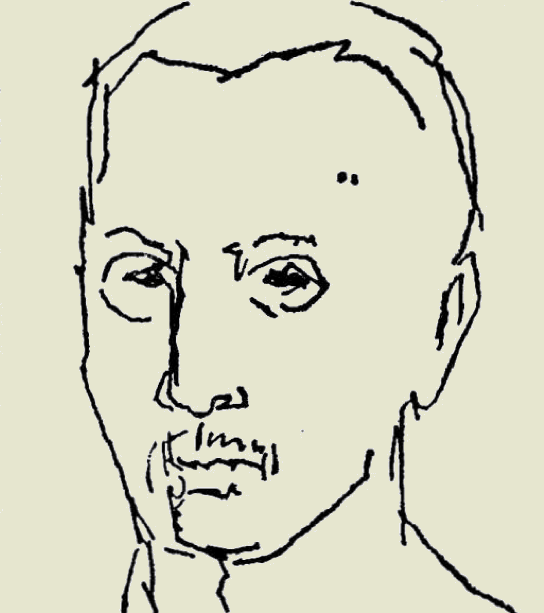
\includegraphics[height=0.9\textheight]{kawahigashi}\\[1em]
        \large{\FS 作~者~像}
    \end{figure}
\end{center}

\newpage

{\FS
    河东碧梧桐(1873—1937),日本爱媛县松山市人,本名秉五郎,又号如月、青桐、桐仙。父亲河东静溪是朱子派学者,在碧梧桐六岁时,就教他读四书五经。碧梧桐于一八八七年入伊予寻常中学,与高滨虚子是同级生。一八九〇年,碧梧桐十八岁时写了俳句集,请正冈子规批改。一八九一年,上东京投考第一高等学校落第。那年夏天,子规回乡省亲,他介绍高滨虚子到子规门下,学作俳句。一八九三年,考入第三高等学校,与虚子同住京都吉田町,宿舍称虚桐庵。次年秋,因学制改革,与虚子转学到仙台第二高等学校,不久与虚子一齐退学,同赴东京,帮助子规提倡俳句革新运动。于是成为子规门下双壁。一八九五年,子规病后,代替子规主持《日本俳句》栏,同年夏,陪子规的母亲去神户探望卧病的子规,并到日本新闻社去工作。翌年,退出日本新闻社,任《新声》杂志的俳句栏主选人。一八九七年,《杜鹃》杂志在松山创刊,负责选句,翌年该杂志移到东京之后,高滨虚子有病,由碧梧桐代替编辑。一九〇二年,搬到子规庵的附近上根岸去住,与子规更亲近,九月子规逝世,继任《日本俳句》的选句人。一九〇三年一月,他再度入日本新闻社,并为《温泉百句》问题,与虚子论战,从这时起,虚子和碧梧桐之间明显地出现了分歧。一九〇五年和一九〇六年,他两度召开「俳三昧」句会,参加者有小泽碧童、大须贺乙字等,专心致意于俳句,切磋琢磨。这时碧派的声势颇大。

    一九〇六年八月六日,经真言宗大谷句佛的资助,开始第一次周游全国。出发前,请高滨虚子接任《日本俳句》的选句工作。他一心渴望此次旅行能有助于使自己的俳境更加深广。翌年在旅次中,他的《新俳句研究谈》出版。一九〇九年四月第二次周游全国,在这一年又进一步阐发新倾向俳句论题。它的特色,可归纳为摆脱羁绊、追求写实、着意心理描写、发挥个性这几点。旅行结束后,他又提出无季自由律,打破俳句的十七音律与季语定型这两个要素,遂变俳句为一般的短诗了。碧梧桐及其对新倾向的俳句的主张,在近代俳句史上打下了划时期的印记,它带着急于开拓的冒进性,脱离了民族文化传统的基础,引起俳界的非议。

    一九二四年碧梧桐建立芜村研究会,为了研究芫村,翌年到与芜村有关的地方旅行,之后,出版了介绍芜村的俳句和绘画的《画人芜村》、《芜村研究》、《芜村新十一部集》、《芜村名句评释》等书。他或许受了赞赏芜村的子规的影响。关于自己的俳句作品和俳论,则有《碧梧桐句集》、《新倾向派俳句的研究》、《三千里》、《续三千里》和《回忆子规》等著作。他的俳风,给人以明快新颖的印象。此外,还编有《续春夏秋冬》、《日本俳句钞》等集子。本集中所选四十五首俳句,都是根据《新订俳句丛书·人与作品》第六卷(樱枫社1980年版)翻译的。
}

\newpage

\section{\FK 春}

\setcounter{haikucounter}{0}

\begin{haiku}
    {\FH ローマの、春の雨になる空よ、窓にすがりて。}

    {\FK 三月三日因病终日闭居}

    {\FK 罗马春雨降,倚窗望天空。\footnote{\FT 碧梧桐文集里,同一标题是另一首俳句「{\FM ミモーザ買はしめて餓ゑて昼眠て}」,此句系某日本网友寻得。}}

    {\FT 注:一九二一年,作者经上海、新加坡,从马赛登陆到意大利罗马等地旅游。六月从巴黎到北欧。十一月到伦敦。十二月渡美,翌年一月回国。}
\end{haiku}

\begin{haiku}
    {\FH \ruby[g]{楠}{くす}の芽に、日のさし風の、光るかな}

    {\FK 日照楠木芽,风吹亦有光。}

    {\FT 注:《楚辞》有「光风」的词儿。}
\end{haiku}

\begin{haiku}
    {\FH 春寒し、水田の上の、\ruby[g]{根}{ね}さし雲。}

    {\FK 早春寒气临,水田上空云无根。}

    {\FT 注:俳人协会故会长大野林火说此句是暗示在悲剧中终了一生的碧梧桐的境涯。句带浪漫味,哀愁美。}
\end{haiku}

\begin{haiku}
    {\FH 曲すみし、\ruby[g]{笛}{ふえ}の\ruby[g]{余音}{よいん}や、春の月。}

    {\FK 横笛一曲终,余音绕春月。}
\end{haiku}

\begin{haiku}
    {\FH 蛇穴を、出でて石\ruby[g]{垣}{がき}の、春の水。}

    {\FK 蛇出洞穴来,石垣春水漾。}

    {\FT 注:句用写生手法,表示敏锐的季节感。}
\end{haiku}

\begin{haiku}
    {\FH \ruby[g]{桐}{きり}の木に、なく\ruby[g]{鶯}{うぐいす}も、茶山哉}

    {\FK 黄莺桐树鸣,茶山多一景。}

    {\FT 注:茶山指春日晴朗时采茶的事,桐树飞来鸣莺,也算多一种景趣。}
\end{haiku}

\begin{haiku}
    {\FH 永き日や、羽\ruby[g]{惜}{おし}む鷹の、嘴使ひ。}

    {\FK 春日迟迟,鹰嘴理毛羽。}

    {\FT 注:作者在此致力于「从平易外观直叙到内面事相与感想具象的描写」。}
\end{haiku}

\begin{haiku}
    {\FH 赤い椿白い椿と落ちにけり。}

    {\FK 红山茶,白山茶,叠地有落花。}

    {\FT 注:此句印象明瞭,如一幅油画,只见地上落下一簇红花,一簇白花,而其场所,使人联想起庭园或山路。这是多被引用、欣赏的名句。}
\end{haiku}

\begin{haiku}
    {\FH 桃咲くや、\ruby[g]{湖}{ご}水のへりの、十個村。}

    {\FK 桃开花似锦,湖水周边十个村。}

    {\FT 注:桃是栽培在农村庭院的花木。此句写桃花开时,瞭望湖边十个村(小村)的艳丽景色。「十个村」用的是汉文。}
\end{haiku}

\section{\FK 夏}

\setcounter{haikucounter}{0}

\begin{haiku}
    {\FH 雪を渡りて、また\ruby[g]{薫風}{くんぷう}の、\ruby[g]{草花}{そうか}\ruby[g]{踏}{ふ}む。}

    {\FK 才行积雪上,又踏熏风草花路。}

    {\FT 注:这里的草花,按《日本的山水》均属于高山植物。句写渡过残雪,又在夏天薰风中踏过花畦,显出爽快明朗、健康的情趣。这是作者在《续三千里》的旅途中,写立山(在富山县西南隅)顶上的即景句。}
\end{haiku}

\begin{haiku}
    {\FH パン屋が出来た、葉櫻の午の、風渡る。}

    {\FK 面包店铺已开业,午问吹渡叶樱风。}

    {\FT 注:叶樱,指樱花开谢后,即长满叶子的樱树。初夏的风一吹,樱树就闪着叶光。此句写郊区商业发达的景象。}
\end{haiku}

\begin{haiku}
    {\FH \ruby[g]{愕然}{がくぜん}として、昼寝さめたる、一人かな。}

    {\FK 愕然昼寝醒,孑立一孤身。}

    {\FT 注:炎夏疲乏,多作午睡。「愕然」用的是汉文。}
\end{haiku}

\begin{haiku}
    {\FH 砲車過ぐる、\ruby[g]{巷}{ちまた}の\ruby[g]{塵}{ごみ}や、日の\ruby[g]{盛}{さか}り。}

    {\FK 炮车驶向巷里过,夏日光中舞沙尘。}

    {\FT 注:此句用新词「炮车」,有时代感。}
\end{haiku}

\begin{haiku}
    {\FH 海楼の、涼しさ\ruby[g]{終}{つ}ひの、別れかな。}

    {\FK 海楼凉气清,惜别此时情。}

    {\FT 注:作者开始「三千里」的旅行,从两国站来到稻毛寄宿于海边松林中的海气馆。门徒乙字、六花、观鱼、碧童等来相送,作此留别句。}
\end{haiku}

\begin{haiku}
    {\FH 馬独り、\ruby[g]{忽}{こつ}と戻りぬ、飛ぶ蛍。}

    {\FK 马儿忽自归,流萤闪烁飞。}
\end{haiku}

\begin{haiku}
    {\FH \ruby[g]{水鶏}{くいな}来し、夜明けて田水、満てるかな。}

    {\FK 水鸡来到黎明前,水淹满田间。}

    {\FT 注:水鸡,身茶褐色、脚长,栖息在芦丛中。黎明前和黄昏时发出像叩门一样的叫声,与「来到」的发音近似。}
\end{haiku}

\begin{haiku}
    {\FH \ruby[g]{温泉}{ゆ}の宿に、馬の子\ruby[g]{飼}{か}へり、\ruby[g]{蠅}{はえ}の声。}

    {\FK 温泉宿舍喂小马,可厌苍蝇声。}

    {\FT 注:小马可爱,蝇声可厌,作者很技巧地把爱与憎凑在一起。}
\end{haiku}

\begin{haiku}
    {\FH 空をはさむ、蟹死にをるや、雲の峰。}

    {\FK 蟹死整钳空,炎天涌云峰。}

    {\FT 注:蟹可能指海蟹。它要钳取什么,终于未能钳着,作者有其寓意。云峰做为死蟹的背景。}
\end{haiku}

\begin{haiku}
    {\FH 薔薇を、けふも書きついで、色の淋しく。}

    {\FK 西光寺寄宿}

    {\FK 书籍放在桌台上,檐前蔷薇放白光。\footnote{\FT 未找到完全对应的句子,怀疑是翻译有误。}}
\end{haiku}

\section{\FK 秋}

\setcounter{haikucounter}{0}

\begin{haiku}
    {\FH 近作を、画室に掛くる、秋日影。}

    {\FK 画室悬近作,秋日光照来。}
\end{haiku}

\begin{haiku}
    {\FH 一軒家も、過ぎ落ちる風の、ままに行く。}

    {\FK 风急吹叶落,陆风过孤屋。}
\end{haiku}

\begin{haiku}
    {\FH 墓と見えて、十字架立つる、秋の山。}

    {\FK 十字架立秋山上,坟墓在望中。}

    {\FT 注:此句用新词「十字架」,带着近代化色彩。}
\end{haiku}

\begin{haiku}
    {\FH 天下知る、\ruby[g]{藏書}{ぞうしょ}見に\ruby[g]{来}{こ}ぬ、秋の晴れ}

    {\FK 藏书名传天下知,来求批览秋晴时。}
\end{haiku}

\begin{haiku}
    {\FH 大風に、傷みし樹々や、渡り鳥。}

    {\FK 大风伤万木,候鸟南归去。}
\end{haiku}

\begin{haiku}
    {\FH 鶴とんで、かえらず池の、水寒。}

    {\FK 萧萧池水寒,鹤飞去不还。}
\end{haiku}

\begin{haiku}
    {\FH 曳かれる牛が、辻でずっと見廻した、秋空だ。}

    {\FK 被牵耕牛停下步,十字路上凝望秋空。}

    {\FT 注:牛被牵走,是到市场呢,还是到屠场?牛也许感到事关自己的命运。此句共计二十三音(七、十一、五),破了调,但有季语「秋空」。}
\end{haiku}

\begin{haiku}
    {\FH から松は、淋しき木なり、赤蜻蛉。}

    {\FK 落叶松寂静,红蜻蜓群舞无声。}

    {\FT 注:此句写晚秋萧瑟静寂的景趣。以落叶松为主,红蜻蜓作陪。俳人碧梧桐与诗人北原白秋的《落叶松》诗境,情感相通。}
\end{haiku}

\begin{haiku}
    {\FH 三日月や、この頃萩の、咲きこぼれ。}

    {\FK 新月刚刚出,胡枝子花零落。}
\end{haiku}

\begin{haiku}
    {\FH この道の、富士になり行く、\ruby[g]{芒}{すすき}かな。}

    {\FK 路径向富士,茫茫狗尾草。}
\end{haiku}

\begin{haiku}
    {\FH 夜に入りて、\ruby[g]{蕃椒}{とうがらし}\ruby[g]{煮}{に}る、臺所。}

    {\FK 时已到夜晚,厨房煮辣椒。}

    {\FT 注:写生活琐事,句法平易,并无陈腐气。子规在《俳句》新派的一种倾向中举了这句。}
\end{haiku}

\begin{haiku}
    {\FH \ruby[g]{芙蓉}{ふよう}見て立つうしろ灯るや。}

    {\FK 伫立看芙蓉,背后点亮灯。}

    {\FT 注:芙蓉是栽培在庭院中的花木,早上开花,傍晚凋萎。此时,室内点起了灯。芙蓉结束了一天的工作,灯火却刚刚点亮,此句写微妙的瞬间变化。}
\end{haiku}

\section{\FK 冬}

\setcounter{haikucounter}{0}

\begin{haiku}
    {\FH 火も置かず、独居の人と、夜長かな。}

    {\FK 夜长不备火,清冷独居人。}
\end{haiku}

\begin{haiku}
    {\FH 夜を寒み、人語聞えて、森の寺。}

    {\FK 寒夜闻人语,庵寺在林中。}
\end{haiku}

\begin{haiku}
    {\FH \ruby[g]{我善坊}{がぜんぼう}に、車引き入れ、ふる霰。}

    {\FK 车入我善坊,玉霰落纷纷。}

    {\FT 注:车是明治时代的人力车,我善坊是谷间的一个町名。霰即常见于初冬时的雪珠。天一阴沉便一小粒一小粒地降落,又叫米雪。}
\end{haiku}

\begin{haiku}
    {\FH 芒枯れし、池に出づ\ruby[g]{工場}{こうば}、さかる\ruby[g]{音}{ね}を。}

    {\FK 漫步到枯芒池畔,风传来工厂噪声。}

    {\FT 注:枯芒是初冬季语,噪音据云可能是木材厂的锯声。}
\end{haiku}

\begin{haiku}
    {\FH 枯木原に、雪積んで居る、月夜かな。}

    {\FK 朦朦月夜,雪封枯木原野。}
\end{haiku}

\begin{haiku}
    {\FH 後宮の、夜半に雪折、聞えけり。}

    {\FK 雪重折枝声,后宫夜半闻。}
\end{haiku}

\begin{haiku}
    {\FH 軒落ちて、雪\ruby[g]{窮}{きゅう}\ruby[g]{巷}{こう}を、\ruby[g]{塞}{ふさ}ぎけり。}

    {\FK 轩前积落雪,贫巷路不通。}

    {\FT 注:据云此句原文是汉语调,系明治俳句的一种特色。}
\end{haiku}

\begin{haiku}
    {\FH 寒林の、貧寺焼けたり、僧の留守。}

    {\FK 寒林贫寺火神来,僧人不知何处去。}
\end{haiku}

\begin{haiku}
    {\FH \ruby[g]{木}{こ}\ruby[g]{枯}{がらし}や、\ruby[g]{谷}{や}中の道を、塔の下。}

    {\FK 大风吹落木,塔下谷中路。}

    {\FT 注:谷中指东京都台东区、上野公园的北部一带,多墓地、寺院和树林。子规的住地根岸离那儿不远。此句系碧梧桐走过那条风吹寒林、落叶飘飞的路时所作。}
\end{haiku}

\begin{haiku}
    {\FH 極月の、風雪\ruby[g]{熊羆}{いうひ}、叫びけり。}

    {\FK 腊月风雪紧,熊罴吼叫声。}
\end{haiku}

\begin{haiku}
    {\FH 灯あかあかと、\ruby[g]{会}{あわ}すれば、千鳥、鳴くといふ。}

    {\FK 会友华灯下,千鸟发鸣声。}

    {\FT 注:写会到意志相投的友人,感到欢欣,以千鸟叫声,作为伴奏。此句打破俳句五、七、五的定型,用六、五、三、五调。}
\end{haiku}

\section{\FK 无季}

\setcounter{haikucounter}{0}

\begin{haiku}
    {\FH 大戦に、\ruby[g]{死所}{ししょ}を得ず\ruby[g]{哀}{あわ}れ、野はかれて。}

    {\FK 读史}

    {\FK 大战未能得死所,悲叹原野尽荒芜。}
\end{haiku}

\begin{haiku}
    {\FH 故人こゝに、在りし遺物と、\ruby[g]{新酒}{しんしゅ}かな。}

    {\FK 怀子规居士旧事}

    {\FK 往昔故人居此处,遗物新酒惹怀思。}
\end{haiku}

\begin{haiku}
    {\FH \ruby[g]{汐}{しお}のよい\ruby[g]{船}{ふな}\ruby[g]{脚}{あし}を瀬戸の\ruby[g]{鷗}{かもめ}は鷗づれ。}

    {\FK 船行潮水好,濑户鸥群竞逐飞。}
\end{haiku}

\chapter[{\FM 高浜虚子}]{\FM \ruby[g]{高}{たか}\ruby[g]{浜}{はま}\ruby[g]{虚}{きょ}\ruby[g]{子}{し}}

\begin{center}
    \begin{figure}
        \centering
        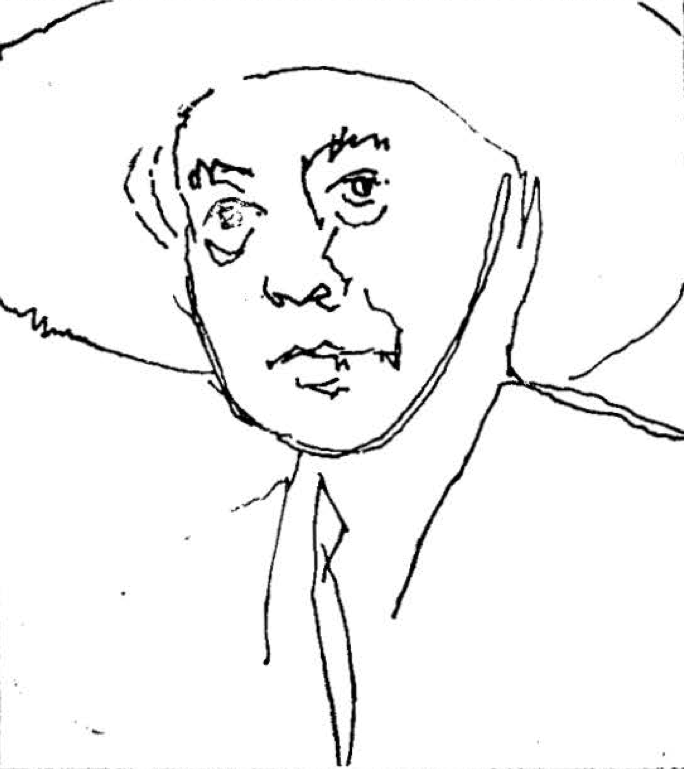
\includegraphics[width=\textwidth]{takahama}\\[1em]
        \large{\FS 作~者~像}
    \end{figure}
\end{center}

\newpage

{\FS
    高滨虚子(1874—1959)生于爱媛县松山市长町新町,本名清。父亲是松山藩士池内庄四郎。废藩设县后,全家搬到风早郡柳原村西下务农。西下家乡风光美好,虚子的童年就在那里度过。父亲爱好谣曲、和歌,母亲也爱好文艺,给虚子很深的影响,从而日后致志于文学工作。八岁时,因四个哥哥均不愿务农,举家又迁回到松山。九岁时,祖母病故,出嗣到祖母家,改姓高滨。一八九一年三月父亲逝世。同年五月伊予寻常中学级友河东碧梧桐(松山人)介绍高滨虚子一起向同乡先辈正冈子规学作俳句。子规以他的本名「清」的谐音,在信里称他为虚子,从此就以虚子作为俳号了。一八九四年虚子与碧梧桐到东京,鼓吹子规所号召的俳句改革主张。翌年冬子规在上野道灌山疗养时,恳请虚子担任俳句革新运动的后继人,但虚子顾虑羁绊太多,婉言辞谢。

    一八九八年一月,《杜鹃》杂志经柳原极堂之手在松山发刊,但因经营不善,由虚子接过来。翌年听子规的建议迁移到东京出版,虚子任发行人,遂面目一新,并培养了不少人才。该刊表现了明治、大正、昭和三代的俳句史的大观。虚子一生的文学活动与《杜鹃》的关系十分密切。子规死后,夏目漱石也给予支持,他的名著《我是猫》,在该刊连载,获得好评。因此刺激了虚子,他也热中于小说的写作,仅一九〇七年一年之内,就在《杜鹃》上发表了《风流忏悔》、《斑鸠故事》、《大内旅馆》等作品。翌年,又将《俳谐师》一作在《国民新闻》上连载。晚年在小诸又写小说《虹》,川端康成给予很高的评价,说虚子是明治以后在艺术上最臻于圆熟的一个人。

    一九〇八年,河东碧梧桐开始提倡俳句新倾向。一九一三年虚子回到俳坛时,写下如下宣言性的俳句:「斗心已抱定,独立丘上迎春风。」他反对新倾向运动,因该运动主张破坏俳句固有的定型,并提倡季题无用论,有发展到无季俳句与自由律的趋势。虚子有自己的俳论,自认为是守旧派。他要维持俳句的结构,说季语不能弃置,与从青年时代就很亲密的碧梧桐对立。在创作方法上,他继承了子规那种客观写生的主张。也就是说,要精细地观察事物,如实地予以描写。题材方面,他主张吟咏花鸟风月,注重自然美。他认为俳句是叙景诗:「俳句的目的,在于吟咏风月。」又说俳句是平俗的诗,俳句是日常的诗……望峻岭、渡大泽,这里有俳句;目见耳闻处,那里有俳句;心感神通处,那里有俳句;太阳出没,寒暑往来,为俳句的根干。他还强调,心情感到悲与喜,应该描写那引起感受的景物。他的注重自然美和日本文艺传统,是有所联系的。他终年八十六,作句又勤,句集浩繁,有独特的风格,有的秀逸轻妙,有的平易纯朴,为广大读者所欢迎。他的文学活动,反映了自己的思想感情,也反映了时代和社会某个角度的情况。由于他多年来在日本俳句等方面的建树,一九五四年十一月获得日本政府颁给的文化勋章。本集中所选一〇八首俳句,都是根据《高滨虚子全集》(共16卷,每日新闻社1974—1975年版)翻译的。
}

\newpage

\section{\FK 新年}

\setcounter{haikucounter}{0}

\begin{haiku}
    {\FH \ruby[g]{去年}{こぞ}\ruby[g]{今年}{ことし}、\ruby[g]{貫}{つらぬ}く棒の、\ruby[g]{如}{ごと}きもの。}

    {\FK 去年与今年,相连如木棍。}

    {\FT 注:这是一九五〇年新年广播的录音句。「去年今年」是俳句的新年季语。作者晚年常说要平凡,他把岁月比作单调的木棍,也可以说是达人达观吧。}
\end{haiku}

\begin{haiku}
    {\FH 手毬唄、悲しきことを、うつくしく。}

    {\FK 悲切手球歌,听来觉得美好。}
\end{haiku}

\begin{haiku}
    {\FH \ruby[g]{琴}{きん}\ruby[g]{棋}{き}\ruby[g]{書}{しょ}\ruby[g]{畫}{が}、松の内なる、遊びかな。}

    {\FK 遣兴松房里,琴棋书画多清趣。}
\end{haiku}

\section{\FK 春}

\setcounter{haikucounter}{0}

\begin{haiku}
    {\FH 春惜む、命惜むに、\ruby[g]{異}{ことな}らず。}

    {\FK 惜春无异惜生命。}

    {\FT 注:一九五〇年作于御苑内霜锦亭举行句会时。}
\end{haiku}

\begin{haiku}
    {\FH 遠ざけて、引寄せもする、春火桶。}

    {\FK 摆出火钵子,春寒闲话时。}
\end{haiku}

\begin{haiku}
    {\FH \ruby[g]{踏}{とう}\ruby[g]{青}{せい}や、古き石\ruby[g]{階}{ばし}、あるばかり。}

    {\FK 踏青呀,只在古旧石阶旁。}

    {\FT 注:踏青是中国的旧俗,三月三日行事,又称踏春,清末梁鼎芬《卜算子》有「只好明年再踏春」之句。}
\end{haiku}

\begin{haiku}
    {\FH 橋に立てば、春水我に、向って来。}

    {\FK 伫立桥头上,春水向我涌来。}
\end{haiku}

\begin{haiku}
    {\FH \ruby[g]{春灯}{しゅんとう}の、下に我あり、\ruby[g]{汝}{いまし}あり。}

    {\FK 华灯春宵里,有我也有你。}
\end{haiku}

\begin{haiku}
    {\FH 春灯、鏡の中の、春灯。}

    {\FK 春灯啊,镜里的春灯。}

    {\FT 注:以反映的手法托出春灯的美。}
\end{haiku}

\begin{haiku}
    {\FH 春潮と、いへば必ず、門司を思ふ。}

    {\FK 提起春潮事,当然想念门司。}

    {\FT 注:春时潮色变作浅蓝,看潮色知道春到来,心情愉快。门司是接联玄海滩与濑户内海的城市,潮景明朗。}
\end{haiku}

\begin{haiku}
    {\FH 春雨に、傘を借りたる、別れかな。}

    {\FK 一八九六年别漱石}

    {\FK 绵绵春雨时,借伞告别离。}
\end{haiku}

\begin{haiku}
    {\FH 思ひ川、渡ればまたも、花の雨。}

    {\FK 渡入思川去,又是花雨天。}

    {\FT 注:思川是地名。}
\end{haiku}

\begin{haiku}
    {\FH 春の山、\ruby[g]{屍}{かばね}を埋めて、\ruby[g]{空}{むな}しかり。}

    {\FK 春山泥土埋尸骨,生前功罪尽虚空。}

    {\FT 注:句意是说春山的草木花鸟仍在,而人的生前是非得失已成一场空。这是凭吊一代之雄源赖朝的。虚子作此句六天后即病逝,也与赖朝一样埋入土中。}
\end{haiku}

\begin{haiku}
    {\FH 独り句の、推敲をして、遅き日を。}

    {\FK 句佛师十七回忌追忆}

    {\FK 春日迟迟,独自推敲句子。}

    {\FT 注:这句是纪念真言宗大谷句佛氏忌辰,写在明信片上的绝笔。}
\end{haiku}

\begin{haiku}
    {\FH 窓外の、風塵春の、行かんとす。}

    {\FK 窗外风尘起,春将归去时。}
\end{haiku}

\begin{haiku}
    {\FH 春風や、\ruby[g]{闘志}{とし}いだきて、丘に立つ。}

    {\FK 斗心已抱定,独立丘上迎春风。}

    {\FT 注:这是一九一三年作者四十岁上回归俳坛时的宣言句。后于一九五〇年又有「斗心尚在见春风」的吟句。}
\end{haiku}

\begin{haiku}
    {\FH 色\ruby[g]{硝子}{ガラス}、\ruby[g]{透}{とお}す春日や、棺の上。}

    {\FK 莎士比亚菩提寺}

    {\FK 春日透过花玻璃,照射棺木上。}
\end{haiku}

\begin{haiku}
    {\FH 春泥の、庭を散歩の、足駄かな。}

    {\FK 漫步庭院里,木屐印春泥。}
\end{haiku}

\begin{haiku}
    {\FH 楊貴妃、という香水の、ありや無しや。}

    {\FK 佳丽杨贵妃,有无点香水?}
\end{haiku}

\begin{haiku}
    {\FH 主婦の頬に、子猫の爪の、痕のあり。}

    {\FK 柏林日本人句会}

    {\FK 主妇脸颊上,小猫脚爪痕。}
\end{haiku}

\begin{haiku}
    {\FH 鶯の、声の大きく、静かさよ。}

    {\FK 群鸟叫声逐渐高,终于静悄悄。}

    {\FT 注:这也是一种写生法,不用眼睛,而用耳朵。此句是时间艺术的表示。}
\end{haiku}

\begin{haiku}
    {\FH 穴を出る、蛇を見て居る、鴉かな。}

    {\FK 乌鸦看着蛇出洞。}
\end{haiku}

\begin{haiku}
    {\FH 江上の、燕は\ruby[g]{緩}{ゆる}く、ボート\ruby[g]{迅}{はや}し。}

    {\FK 燕子江天缓缓飞,船行何迅速。}
\end{haiku}

\begin{haiku}
    {\FH 鶯や、文字も知らずに、歌心。}

    {\FK 黄莺不识文字,却有歌吟的心。}
\end{haiku}

\begin{haiku}
    {\FH 蝶飛や、蘇山人の魂、遊ぶらん。}

    {\FK 飞蝶悠悠,岂是苏山人魂游。}

    {\FT 注:苏山人是作者的俳友,见正冈子规「春雨霏霏」句的注释。}
\end{haiku}

\begin{haiku}
    {\FH 門内の、庭の広さや、蚕飼宿。}

    {\FK 门前两亩桑,好把蚕来养。}
\end{haiku}

\begin{haiku}
    {\FH \ruby[g]{海女}{あま}とても、\ruby[g]{陸}{くが}こそよけれ、桃の花。}

    {\FK 渔女登上陆地,恍似桃花艳丽。}

    {\FT 注:一九四八年虚子游览三重县志摩时,看到外海渔女潜水采贝的作业,即作此句。操渔女作业的,多从少女时开始,她们登陆休息时焚火取暖,吃饭笑谈,也有给婴孩喂奶者。作者为渔女表示祝福之意,同时,又产生像桃花报南国之春的美感。}
\end{haiku}

\begin{haiku}
    {\FH 山居杉に、\ruby[g]{親}{した}しめば、\ruby[g]{連翹}{れんぎょう}野に恋し}

    {\FK 山居爱杉树,又恋连翘野原。}
\end{haiku}

\begin{haiku}
    {\FH 花見にと、馬に\ruby[g]{鞍}{くら}置く、心あり。}

    {\FK 马背挂雕鞍,神往到花前。}

    {\FT 注:此句取材谣曲《马挂鞍》。花即樱花。}
\end{haiku}

\begin{haiku}
    {\FH 倫敦の、\ruby[g]{春草}{しゅんそう}を踏む、我が草履。}

    {\FK 我的芒鞋哟,踩着伦敦的春草。}

    {\FT 注:作者旅欧时,穿和服与草鞋,是引人注目的。}
\end{haiku}

\begin{haiku}
    {\FH 初蝶\ruby[g]{来}{く}、何色と\ruby[g]{問}{と}ふ、\ruby[g]{黄}{き}と答ふ。}

    {\FK 蝴蝶翩翩新到来,问何颜色答说黄。}

    {\FT 注:在这首俳句里面,有如闻其声的来、问、答三段对话,黄是三月间的花色。这是虚子作于信州小诸的名句。}
\end{haiku}

\begin{haiku}
    {\FH 一つ根に、離れ\ruby[g]{浮}{う}く葉や、春の水。}

    {\FK 荇藻飘浮春水面,两叶分离根一条。}

    {\FT 注:这是写生的典型手法的例句。}
\end{haiku}

\begin{haiku}
    {\FH 鎌倉の、古き土より、牡丹の\ruby[g]{芽}{め}。}

    {\FK 镰仓故土上,吐出牡丹芽。}
\end{haiku}

\begin{haiku}
    {\FH ---}

    {\FK 伫立花前不见花。\footnote{\FT 未找到此句。}}
\end{haiku}

\begin{haiku}
    {\FH 花散るや、鈍な鴉の、翅あたり。}

    {\FK 樱花瓣飘散,落在乌鸦钝翅膀。}

    {\FT 注:樱花的白瓣和乌鸦的黑翅膀,形成鲜明的对照,显出古典美。使人联想到李商隐的诗句「紫鸾不肯舞,满翅蓬山雪」(《海上谣》)。描写白雪落在紫鸾的翅膀上,当各有其讽托之意。}
\end{haiku}

\begin{haiku}
    {\FH 散る花を、悼む心も、\ruby[g]{慌}{あわただ}し。}

    {\FK 哀花谢落心零乱。}

    {\FT 注:一九四一年四月二十一日虚子哀悼维子郎逝世句。}
\end{haiku}

\begin{haiku}
    {\FH 此の谷の、梅の\ruby[g]{遅速}{ちそく}を、獨り\ruby[g]{占}{し}む}

    {\FK 不管梅开快与慢,独占此谷间。}
\end{haiku}

\begin{haiku}
    {\FH 金堂の、扉を\ruby[g]{叩}{たた}く、木の芽風。}

    {\FK 树芽风,敲打金堂门。}
\end{haiku}

\begin{haiku}
    {\FH ---}

    {\FK 漂动急湍里,荇菜生机旺。\footnote{\FT 未找到此句。}}
\end{haiku}

\begin{haiku}
    {\FH \ruby[g]{自}{みずか}ら草といい\ruby[g]{芳草}{ほうそう}といわず。}

    {\FK 祝《草》三十五周年纪念}

    {\FK 自云是小草,不愿称瑶香。}
\end{haiku}

\section{\FK 夏}

\setcounter{haikucounter}{0}

\begin{haiku}
    {\FH 虹立ちて、\ruby[g]{忽}{たちま}ち君の、\ruby[g]{在}{あ}る\ruby[g]{如}{ごと}し。}

    {\FK 长虹挂彩,忽想如君在。}
\end{haiku}

\begin{haiku}
    {\FH 虹消えて、忽ち君の、\ruby[g]{無}{な}き如し。}

    {\FK 彩虹淌逝,忽想如君去。}

    {\FT 注:虚子旅居小诸,看见彩虹挂在浅间山顶,一九四四年十一月七日,在明信片上写下这两句给住在福井县的女弟子森田爱子。后用在他的小说《虹》的末尾。}
\end{haiku}

\begin{haiku}
    {\FH 夕立や、ぬれて戻りて、欄に\ruby[g]{倚}{よ}る。}

    {\FK 骤雨身淋湿,归来独倚栏。}

    {\FT 注:此句系陪送正冈子规到须磨疗养院后所作。}
\end{haiku}

\begin{haiku}
    {\FH 夕立や、森を出で来る、馬車一つ。}

    {\FK 黄昏骤雨降,马车一驾出林来。}
\end{haiku}

\begin{haiku}
    {\FH 夏海や一帆の又見え来る。}

    {\FK 长夏海面上,又见风帆一叶来。}
\end{haiku}

\begin{haiku}
    {\FH 晩涼に、池の\ruby[g]{萍}{うきくさ}、皆動く。}

    {\FK 一阵晚凉风,满池萍叶动。}

    {\FT 注:「晚凉」用汉语。白居易有「绿树阴前逐晚凉」句。}
\end{haiku}

\begin{haiku}
    {\FH 夏潮の、今\ruby[g]{退}{そ}く平家、\ruby[g]{亡}{ほろ}ぶ時も。}

    {\FK 夏潮今退去,平家灭亡时。}

    {\FT 注:这是咏史句。源义经在坛浦利用夏潮,指挥军船迫近平家的军船,瞬息之间决定了胜利。现在门司布刈神社有此句碑。}
\end{haiku}

\begin{haiku}
    {\FH 立山の、其連峰の、雪解水。}

    {\FK 悼下村为山}

    {\FK 立山巉岩上,夏雪正消溶。}
\end{haiku}

\begin{haiku}
    {\FH 静に居、\ruby[g]{団扇}{うち}の風も、たまに好し。}

    {\FK 静静听说笑,悠悠团扇摇。}
\end{haiku}

\begin{haiku}
    {\FH ---}

    {\FK 芭蕉洒了水,卷叶冲上天。\footnote{\FT 未找到此句。}}
\end{haiku}

\begin{haiku}
    {\FH 夕嵐、青\ruby[g]{鷺}{さぎ}吹き去って、高楼に灯。}

    {\FK 青鹭已随晚风去,高楼犹有灯火明。}

    {\FT 注:青鹭是大型鹭鸟,背苍灰色,故名。成群地在水边的树上作巢,喜在清凉的水中伫立。}
\end{haiku}

\begin{haiku}
    {\FH 蜘蛛に\ruby[g]{生}{あ}れ、\ruby[g]{網}{あみ}をかけねば、ならぬかな。}

    {\FK 生为蜘蛛,就该结网啊!}

    {\FT 注:这种意识形态,也是一种人生论。}
\end{haiku}

\begin{haiku}
    {\FH 蜘蛛網を、張るが如くに、我もあるか。}

    {\FK 像蜘蛛结网,我也是吗?}

    {\FT 注:一种人生论,在俳句这小体裁单纯地表现出来。}
\end{haiku}

\begin{haiku}
    {\FH 夏の蝶、日かげ日なたと、飛びにけり。}

    {\FK 夏天蝴蝶飞翔,向阴又向阳。}
\end{haiku}

\begin{haiku}
    {\FH 山国の、蝶をあらしと、思はずや。}

    {\FK 真没想到呀,搅乱了山区蝴蝶!}

    {\FT 注:一九四五年五月虚子沿着浅间山斜坡的田野路行走时,看见路两旁开着豌豆花,而蝴蝶群却飞得很慌乱,原来是被美军大轰炸吓的。这是对同行人顺口吟出之句,为代表作之一。}
\end{haiku}

\begin{haiku}
    {\FH 夏蝶の、つと落ち\ruby[g]{来}{きた}り,とび\ruby[g]{翔}{かけ}り。}

    {\FK 嬉戏落花地,蝴蝶追逐蝴蝶。}
\end{haiku}

\begin{haiku}
    {\FH \ruby[g]{金}{こ}\ruby[g]{亀子}{がねむし}、\ruby[g]{擲}{なげう}つ闇の、深さかな。}

    {\FK 扔掉的金龟子,飞入黑暗深处。}

    {\FT 注:金龟子,夏天甲虫,白天藏在草木荫处,夜间出来绕着灯火飞动。}
\end{haiku}

\begin{haiku}
    {\FH 螢灯の、傷つき落つる、水の上。}

    {\FK 萤火虫受了伤,跌落水面上。}
\end{haiku}

\begin{haiku}
    {\FH \ruby[g]{主客}{しゅかく}\ruby[g]{閑話}{かんわ}、ででむし竹を、上るなり。}

    {\FK 宾主在谈天,蜗牛爬上竹竿。}
\end{haiku}

\begin{haiku}
    {\FH 我を見て、\ruby[g]{舌}{した}を出したる、大\ruby[g]{蜥蜴}{とかげ}。}

    {\FK 这只大蜥蜴,吐出舌尖看着我。}

    {\FT 注:大蜥蜴吐舌的怪模样,使作者苦笑地对着它。}
\end{haiku}

\begin{haiku}
    {\FH 山を出でて、山に入る月や、蚊帳の外。}

    {\FK 蚊帐外,月儿出山又入山。}
\end{haiku}

\begin{haiku}
    {\FH 蚊帳越しに、\ruby[g]{薬}{やく}煮る母を、かなしみつ。}

    {\FK 掀开蚊帐,愁看煎药的母亲。}
\end{haiku}

\begin{haiku}
    {\FH 薔薇剪って、短き詩をぞ、作りける。}

    {\FK 修剪蔷薇时,兴起吟短诗。}
\end{haiku}

\begin{haiku}
    {\FH \ruby[g]{藻}{も}の花を、かづいて出でし、泳ぎかな。}

    {\FK 戴上水藻花,出去游泳啦。}

    {\FT 注:藻草生在湖泊水底,绿叶蹿出水面。夏天,叶间绽开淡绿、黄、白等色的花。}
\end{haiku}

\begin{haiku}
    {\FH 牡丹の、一弁落ちぬ、俳\ruby[g]{諧}{かい}史。}

    {\FK 俳谐史上,掉落牡丹一瓣。}

    {\FT 注:此句是追悼俳人松本氏的逝世。因松本氏的人品、句品均佳,作者把他比作白牡丹的一瓣。}
\end{haiku}

\begin{haiku}
    {\FH 夕顔の、花に涙を、流すかな。}

    {\FK 子规病笃}

    {\FK 滴滴泪水,落在瓠瓜花蕊。}

    {\FT 注:此句作于一九〇一年二七月。瓠瓜,日本称夕颜,原产于美国\footnote{{\FT 瓠瓜和夕颜实为葫芦,学名} \textit{Lagenaria siceraria}{\FT ,原产于非洲。}}。茎叶有软毛,晚间开白花,翌晨即凋萎。子规院子里,有个作药用的瓠瓜棚,故这么说。}
\end{haiku}

\section{\FK 秋}

\setcounter{haikucounter}{0}

\begin{haiku}
    {\FH 手で顔を、撫づれば鼻の、冷たさよ。}

    {\FK 伸手一摸脸,鼻子好凉呦。}

    {\FT 注:句自然浅白,又稍带幽默感。这是虚子的另一种句式。}
\end{haiku}

\begin{haiku}
    {\FH 秋風や、眼中のもの、皆俳句。}

    {\FK 秋风吹拂凉,眼中万物皆诗章。}
\end{haiku}

\begin{haiku}
    {\FH 霧の中に、蓑の人現れ、又隠れぬ。}

    {\FK 雾里蓑衣人,乍现又乍隐。}
\end{haiku}

\begin{haiku}
    {\FH 百花園、野分の跡を、見に来たり。}

    {\FK 来到百花园里,巡视大风过后痕迹。}
\end{haiku}

\begin{haiku}
    {\FH 昴明く、銀河の暗き、ところあり。}

    {\FK 银河无踪影,只有月亮和昴星。}
\end{haiku}

\begin{haiku}
    {\FH 秋の雲、\ruby[g]{太虚}{たいきょ}の風に、乗りにけり。}

    {\FK 秋空一片云,悠闲漫步行。}
\end{haiku}

\begin{haiku}
    {\FH 大いなる、月を簾に、\ruby[g]{印}{しる}しけり。}

    {\FK 大圆月,印在门帘上。}
\end{haiku}

\begin{haiku}
    {\FH これよりは、山陰道の、月暗し。}

    {\FK 悼山本村家}

    {\FK 山阴道上,今后月暗淡。}
\end{haiku}

\begin{haiku}
    {\FH 草の露、三千人の、涙かな。}

    {\FK 子规七七忌追悼句会}

    {\FK 草上露,三千人的泪珠。}
\end{haiku}

\begin{haiku}
    {\FH 虚子一人、銀河と共に、西へ行く。}

    {\FK 虚子单身,随银河西行去。}

    {\FT 注:此句有向往西方净土的佛家思想。作者还有「寝中寂静,唯有银河流水声」的想象句。}
\end{haiku}

\begin{haiku}
    {\FH \ruby[g]{仲麿}{なかまろ}の、舟は波間や、天の川。}

    {\FK 浪里晁衡船,天河腾翻。}

    {\FT 注:此是怀古句。日本人晁衡从长安回国途中,在海上遇大风浪,辗转折回长安。李白有诗怀念他,}
\end{haiku}

\begin{haiku}
    {\FH 船に乗れば、陸\ruby[g]{情}{なさ}けあり、暮の秋。}

    {\FK 暮秋扬帆去,我念陆地情。}

    {\FT 注:一九一八年十月为纪念亡兄逝世三周年,在回乡的途中所作。虽说客观写生,却是主观抒情句。}
\end{haiku}

\begin{haiku}
    {\FH \ruby[g]{病}{わくら}葉や、大地に何の、病ある。}

    {\FK 大地染何疾?病叶尽飘零。}
\end{haiku}

\begin{haiku}
    {\FH \ruby[g]{爛}{らん}々と、昼の星見え、\ruby[g]{菌}{きの}生え。}

    {\FK 火星何灿烂,蘑菇妖艳生。}

    {\FT 注:原文「昼星」,依山本健吉作「火星」解,故照译。此句写秋空星光灿烂,而地下的蘑菇红黄妖艳,天上地下,不同色彩,形成鲜明对照。}
\end{haiku}

\begin{haiku}
    {\FH \ruby[g]{来}{こ}ん秋を、再び期して、別れけり。}

    {\FK 此刻一为别,来秋期再会。}
\end{haiku}

\begin{haiku}
    {\FH \ruby[g]{落花生}{らっかせい}、喰ひつゝ読むや、罪と罰。}

    {\FK 边吃花生边阅读,《罪与罚》那本书。}
\end{haiku}

\begin{haiku}
    {\FH 彼一語、我一語秋、深みかも。}

    {\FK 他一言,我一语,不觉秋已深。}

    {\FT 注:写在宾主愉快交谈时,室外日己斜,落叶也飘舞了,这是寄喻人生到了秋深的时节。}
\end{haiku}

\begin{haiku}
    {\FH 月を思い、人を思ひて、須磨にあり。}

    {\FK 客居须磨浦,怀月又怀人。}

    {\FT 注:须磨在神户西部南海岸。《源氏物语》的主人公光源氏曾被谪在此,这里的月亮照过历史上多少豪杰。虚子于五十多年前陪送正冈子规到此地疗养,曾一起赏月,不禁引起追怀。}
\end{haiku}

\begin{haiku}
    {\FH 落葉降り、やがて雪降り、霰降り。}

    {\FK 落叶飘下,接着雪飘下,霰飘下。}

    {\FT 注:此句写自然规律,也有人生飘忽之感。}
\end{haiku}

\begin{haiku}
    {\FH \ruby[g]{案}{あん}\ruby[g]{山}{ざん}\ruby[g]{子}{し}、我に向ひて、問答す。}

    {\FK 稻草人向我搭话。}
\end{haiku}

\begin{haiku}
    {\FH ひらひらと、\ruby[g]{釣}{つ}られて淋し、今年\ruby[g]{鯊}{はぜ}。}

    {\FK 江中木桩上,独坐钓鲨鱼\footnote{\FT 这里的鲨鱼实际是虾虎鱼。}。}
\end{haiku}

\begin{haiku}
    {\FH 胸出して、\ruby[g]{鳩}{はと}のぼり來る、落葉坂。}

    {\FK 鸽子胸挺挺,登上落叶坡。}
\end{haiku}

\begin{haiku}
    {\FH わが\ruby[g]{庵}{いお}の、椿に\ruby[g]{鵯}{ひよ}の、来る日課。}

    {\FK 我家山茶树一棵,鹎鸟探花当日课。}

    {\FT 注:鹎系鸣禽类,形似画眉,善飞翔,飞时一上一下波状地向前。}
\end{haiku}

\begin{haiku}
    {\FH この松の、下にたゝすめは、露のわ\ruby[g]{連}{つら}。}

    {\FK 伫立此松下,露之中。}

    {\FT 注:在风早村西下家乡的屋子旁边,有一棵老松树,虚子幼时常在松树下玩耍。隔了三十多年回乡再看时,老松依然耸立,难兔有所追怀。表示人在露中,从露又联想到泪,有点感伤。}
\end{haiku}

\begin{haiku}
    {\FH 桐一葉、日当りながら、落ちにけり。}

    {\FK 桐树日光照,枝梢一叶飘。}

    {\FT 注:写出天地幽玄的信息,一叶落而知秋。虚子名句之一。}
\end{haiku}

\begin{haiku}
    {\FH 大江の、両岸の蘆、刈るとかや。}

    {\FK 大江两岸,芦苇割掉了吗?}
\end{haiku}

\begin{haiku}
    {\FH 柳散り、蓮破れ、お濠尚存す。}

    {\FK 荷残柳败城池在。}
\end{haiku}

\begin{haiku}
    {\FH ---}

    {\FK 苹果未吃完,放在手册上。\footnote{\FT 未找到此句。}}
\end{haiku}

\begin{haiku}
    {\FH 枯菊の、色\ruby[g]{尚}{なお}\ruby[g]{存}{そん}す、霜の庭。}

    {\FK 菊残色尚美,犹立风霜庭院里。}
\end{haiku}

\section{\FK 冬}

\setcounter{haikucounter}{0}

\begin{haiku}
    {\FH 遠山に、日の当りたる、枯野かな。}

    {\FK 举目远山前,薄日照荒原。}

    {\FT 注:这是早期在虚子庵例会上作的俳句。冬天的日光令人感到温暖。此句是作者喜爱的代表作之一。}
\end{haiku}

\begin{haiku}
    {\FH 傘さして、ゆくや枯野の、雨の音。}

    {\FK 携伞向前行,枯野听雨声。}
\end{haiku}

\begin{haiku}
    {\FH ---}

    {\FK 寒夜出当铺,仰观岁暮月。\footnote{\FT 未找到此句。}}
\end{haiku}

\begin{haiku}
    {\FH 眠れねば、いろいろの智慧、夜半の冬。}

    {\FK 醒来冬夜半,慧想起联翩。}
\end{haiku}

\begin{haiku}
    {\FH 二行書き、一行\ruby[g]{消}{け}すや、寒灯下。}

    {\FK 寒灯下,写两行删一行。}
\end{haiku}

\begin{haiku}
    {\FH 寒潮に、\ruby[g]{河豚}{ふぐ}の毒を、洗ひけり}

    {\FK 就在寒潮里,河豚毒洗去。}
\end{haiku}

\begin{haiku}
    {\FH \ruby[g]{鳰}{にお}がゐて、鳰の海とは、昔より。}

    {\FK 浮游䴙䴘在,自古便称䴙䴘海。}

    {\FT 注:琵琶湖的湖面有点点的水鸟䴙䴘,故称䴙䴘海。《万叶集》中有柿本人麻吕的短歌:「䴙䴘海波涌,黄昏千鸟鸣,汝鸣吾有感,思古发幽情。」松尾芭蕉有俳句:「四方飘下花雪来,尽归䴙䴘海。」一九三九年秋,虚子在琵琶湖饭店作此句,抒发怀古之情。}
\end{haiku}

\begin{haiku}
    {\FH 鴨の中の、一つの鴨を、見てゐたり。}

    {\FK 在鸭群里,单看着一只。}
\end{haiku}

\begin{haiku}
    {\FH 水鳥の、夜半の羽音や、あまたたび。}

    {\FK 时已到深更,水鸟屡发拍翅声。}

    {\FT 注:写大静中小动的声音,稍显出幽玄感。}
\end{haiku}

\begin{haiku}
    {\FH 鳴くたびに、枝踏みゆるゝ、寒鴉。}

    {\FK 寒鸦鸣叫时,跳踏着树枝。}
\end{haiku}

\begin{haiku}
    {\FH 大根を、\ruby[g]{鷲}{わし}づかみにし、五六本。}

    {\FK 大鹫抓萝卜,五六根。}
\end{haiku}

\begin{haiku}
    {\FH 流れ行く、大根の葉の、早さかな。}

    {\FK 川上萝卜叶,急速漂流去。}

    {\FT 注:作者在小川的桥上,看见水上萝卜叶很快地流去,就照实况吟出那瞬间的情趣。}
\end{haiku}

\begin{haiku}
    {\FH 浦嶋草、一夜の霜に、老いにけり。}

    {\FK 离离浦岛草,霜中一夜即衰老。}
\end{haiku}

\chapter[{\FM 水原秋櫻子}]{\FM \ruby[g]{水}{みず}\ruby[g]{原}{はら}\ruby[g]{秋}{しゅう}\ruby[g]{櫻}{おう}\ruby[g]{子}{し}}

\begin{center}
    \begin{figure}
        \centering
        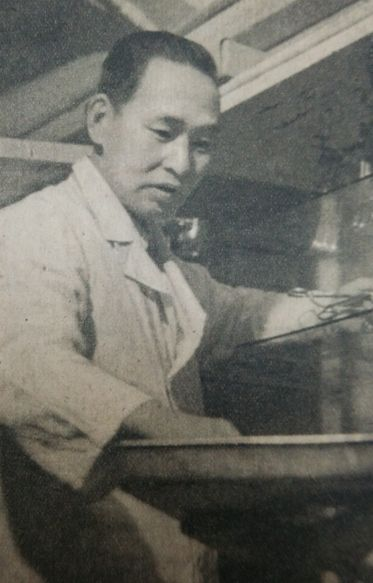
\includegraphics[height=0.9\textheight]{mizuhara}\\[1em]
        \large{\FS 作~者~像}
    \end{figure}
\end{center}

\newpage

{\FS
    水原秋樱子(1892—1982),生于东京神田猿乐町,本名丰,别号喜雨亭。父熊三郎,母治子,秋樱子是长子。学历是东京高师附属小学校、德国学协会中学,二十岁入第一高等学校。这时爱读歌集。一九一八年毕业于东京帝国大学医学部。在校时吟咏短歌。后获得医学博士学位,并任昭和医专教授。他经营过妇产科病院,还在宫内省侍医寮任过职。一九一八年他接触高滨虚子的俳句论文,对俳句发生兴趣,遂购读《杜鹊》杂志。翌年在血清化学教室的先辈绪方春桐的劝告下开始作句,入了树芽会,俳号静夏。因该会领导人南仙卧、野村喜舟等的缘故,出席《涩柿》俳句会,不满意于松根东洋城对写生法的指导,改向《杜鹃》杂志投稿,在例会上初次见高滨虚子。那时期,医学先辈宇都野研办《朝光》歌志,劝秋樱子向窪田空穗学习短歌,作歌入选。一九二二年与山口誓子、日野草城、富安风生、高野素十、山口青邨等建立东大俳句会,给《杜鹃》吹入一股新风。由于秋樱子、誓子、素十、青邨这四个活跃的人物,名字用拉丁文拼出来的话,字头都是S,昭和初期的《杜鹃》杂志遂出现了四S时代。

    一九二二年,秋樱子加入佐佐木绫华主宰的《破魔弓》,被推选为选者。一九二八年七月该杂志改名为《马醉木》,长期由秋樱子主持职务。关东大地震后,秋樱子不再写短歌,致力于俳句,到全国名胜旅游,感兴作句。此后,反对《杜鹃》上的那些陷于烦琐描写的客观写生。一九三一年十月,在《马醉木》发表名文《自然的真与文艺的真》,脱离了《杜鹃》杂志社。他认为自然的真不等于艺术上的真,自然的真不过是一种素材,需要作者琢磨,主观的沉浸,获得艺术的旨趣,而达到自由抒情的目的。他既不赞同作句如实的客观写生,也不愿意停留在花鸟的吟咏上。要求清新活泼,导入短歌抒情表现,树立主观写生。

    对连作俳句的倡导后来引起了新兴俳句运动,环绕着季题存废问题,俳坛上展开了争论。秋樱子批判无季和口语化的倾向,坚持有季,定型,使用文语。一九六二年五月就任俳人协会会长、一九七八年任名誉会长。一九六四年获得日本艺术院奖,一九六六年被推选为日本艺术院会员。

    他的著作甚丰,包括《葛饰》、《新树》、《秋苑》、《浮叶抄》等句集,俳论、随笔、纪行、日记等。为纪念他而建立的句碑约有三十座。本集中所选一一四首俳句,都是根据《水原秋樱子全集》(共21卷,讲谈社1979年版)翻译的。
}

\newpage

\section{\FK 新年}

\setcounter{haikucounter}{0}

\begin{haiku}
    {\FH 獅子舞は、入日の富士に、手をかざす。}

    {\FK 狮子舞到日落西,额手拟欲观富士。}

    {\FT 注:狮子舞是神乐之一种,为驱邪祝福,正月挨门逐户舞蹈。}
\end{haiku}

\begin{haiku}
    {\FH \ruby[g]{元日}{がんじつ}や、鷹がつらぬく、丘の空。}

    {\FK 元旦老鹰飞翔,穿入丘陵云天。}
\end{haiku}

\begin{haiku}
    {\FH 千鳥ゐて、初日の川を、舟行かず。}

    {\FK 元旦川上不行船,千鸟飞于天。}
\end{haiku}

\begin{haiku}
    {\FH 田にゐたる、鴨が初日を、よぎり飛ぶ。}

    {\FK 元日耀晨曦,田间野鸭横飞去。}

    {\FT 注:冰冻的沼田、元日在晨曦映照之下,一只野鸭倏地横飞过去。}
\end{haiku}

\begin{haiku}
    {\FH 一輪の、霜の薔薇より、年\ruby[g]{明}{あ}くる。}

    {\FK 比起一朵霜蔷薇,新岁更芳菲。}
\end{haiku}

\section{\FK 春}

\setcounter{haikucounter}{0}

\begin{haiku}
    {\FH \ruby[g]{万葉}{まんよう}に、東歌あり、\ruby[g]{紀元節}{きげんせつ}。}

    {\FK 纪元佳节日,口诵《万叶·东歌》。}

    {\FT 注:纪元节,即二月十一日,是神武天皇在橿原宫登基的日子。战后一度废除,一九六六年改为建国纪念日。《东歌》为《万叶集》第十四卷的标题,收集和歌二三〇首,素朴地表现古代东部各地人民的生活和别离的痛苦。}
\end{haiku}

\begin{haiku}
    {\FH \ruby[g]{春日野}{かすがの}の、藤を\ruby[g]{華鬘}{けまん}と、なしたまふ。}

    {\FK 伎艺天女}

    {\FK 春日野藤萝,采编做华鬘。}

    {\FT 注:华鬘是印度风俗,以线串花朵,装饰头部或身体。}
\end{haiku}

\begin{haiku}
    {\FH 凧の絵の、\ruby[g]{舳艫}{じくろ}\ruby[g]{赤壁}{せきへき}の、峡に満つ。}

    {\FK 舳舻风筝绘,布满赤壁峡。}

    {\FT 注:此句写曹操下江南军容。}
\end{haiku}

\begin{haiku}
    {\FH 朝寝せり、\ruby[g]{孟}{もう}\ruby[g]{浩}{こう}\ruby[g]{然}{ぜん}を、始祖として。}

    {\FK 清晨贪睡眠,始祖乃是孟浩然。}

    {\FT 注:唐诗人孟浩然有「春眠不觉晓」句,故作者奉为始祖,他自己乃是后辈。}
\end{haiku}

\begin{haiku}
    {\FH 残る雪、月黄なる夜を、\ruby[g]{失}{う}せにけり。}

    {\FK 月色朦胧夜,残雪已消去。}

    {\FT 注:这是作者在某夜归迟,见自宅山毛榉下残雪消溶的即景句。}
\end{haiku}

\begin{haiku}
    {\FH ---}

    {\FK 梅影印家门,夜夜月。\footnote{\FT 未找到此句。}}
\end{haiku}

\begin{haiku}
    {\FH 古鏡見る、窓前梅の、さかりなり。}

    {\FK 眼观古镜里,窗前梅盛开。}

    {\FT 注:此句令人喜爱,用的是「返照」手法。作者在陈列室看到古镜,也看到窗外梅花,把它们联系起来描写,并表达愉快的心情。}
\end{haiku}

\begin{haiku}
    {\FH 春一番、武蔵野の池、波あげて。}

    {\FK 春来武藏野,初次吹皱池水。}
\end{haiku}

\begin{haiku}
    {\FH べたべたに、田も菜の花も、照りみだる。}

    {\FK 雨田湿,菜花黄,黏黏糊糊光影乱。}

    {\FT 注:一九五〇年作者往来横滨在小机站,瞭望风光。此句有印象画派那种光色鲜艳的风格。}
\end{haiku}

\begin{haiku}
    {\FH \ruby[g]{渦}{うず}\ruby[g]{群}{む}れて、\ruby[g]{暮春}{ぼしゅん}海景、あらたまる。}

    {\FK 涡潮阵阵,暮春海景更新。}

    {\FT 注:作者到大毛岛看到鸣门的涡潮,以为暮春海景全变了。}
\end{haiku}

\begin{haiku}
    {\FH 行春や、娘\ruby[g]{首}{がしら}の、髪の\ruby[g]{艶}{つや}。}

    {\FK 春将去时,姑娘头发艳丽。}

    {\FT 注:这里姑娘指手托的木偶姑娘,头发染过,看来很美。作者在德岛市木偶师的工作室所见的即景句。}
\end{haiku}

\begin{haiku}
    {\FH 高\ruby[g]{嶺}{ね}星、\ruby[g]{蚕飼}{こがい}の村は、寝しづまり。}

    {\FK 闪烁高岭星,沉睡养蚕村。}
\end{haiku}

\begin{haiku}
    {\FH ---}

    {\FK 疾风吹过来,春禽倒在田界。}

    {\FT 注:春禽即矮鸡,一种供玩赏的小鸡。\footnote{\FT 未找到此句。}}
\end{haiku}

\begin{haiku}
    {\FH 燕来て、山家に鳴けば、春祭。}

    {\FK 燕子飞鸣到山家,正是春祭时节。}
\end{haiku}

\begin{haiku}
    {\FH 春月や、寝鳥のたちし、\ruby[g]{雑}{ぞう}木原。}

    {\FK 春月映照杂树原,宿鸟惊飞起。}

    {\FT 注:这是行吟句。春月夜,作者偕友外出,归途中经过杂树的丘原,脚步声惊醒了睡着的鸟儿,忽然从巢里飞出。}
\end{haiku}

\begin{haiku}
    {\FH 谷深く、うぐいす鳴けり、夕霞。}

    {\FK 深谷莺声美,晚霞照眼明。}
\end{haiku}

\begin{haiku}
    {\FH 鶯や、\ruby[g]{前}{さき}山いよよ、雨の中。}

    {\FK 前山莺鸟啼,濛濛雨中天。}
\end{haiku}

\begin{haiku}
    {\FH \ruby[g]{鴛鴦}{おし}のゐて、波をつくるよ、花の影。}

    {\FK 鸳鸯漫游划波纹,水面樱花影。}

    {\FT 注:此句写四月的景色,一幅华丽的花鸟画。}
\end{haiku}

\begin{haiku}
    {\FH 雨に\ruby[g]{獲}{え}し、白魚の\ruby[g]{嵩}{かさ}、\ruby[g]{哀}{あわ}れなり。}

    {\FK 雨中获白鱼,深沉哀悼意。}

    {\FT 注:旧时德川家康爱白鱼,命家臣从伊势移植到隅田川,取得成功。至今隅田川为白鱼的名所。在春雨迷濛的水天背景中,用网捕到白鱼。作者怜惜眼前的白鱼,并对门徒宫城二郎表示哀悼。这句是作者应二郎的父亲之邀乘船到川上捕白鱼时所作。}
\end{haiku}

\begin{haiku}
    {\FH 菓子買ひに、妻をいざなふ、地虫の夜。}

    {\FK 蛴螬夜鸣时,邀妻买糕饼去。}

    {\FT 注:写晚春之夜,地虫鸣叫时,劝爱妻一道去买洋点心,就势儿散散步。}
\end{haiku}

\begin{haiku}
    {\FH \ruby[g]{蟇}{ひき}ないて、\ruby[g]{唐招提寺}{とうしょうだいじ}、春いづこ。}

    {\FK 蟾蜍鸣叫招提寺,春归何处去?}

    {\FT 注:唐招提寺在奈良五条,寺内有鉴真和尚雕像。作者怀着感慨今昔的心情,不见唐招提寺春天的佳景,只听蟾蜍的叫声,不禁要问春归何处去。}
\end{haiku}

\begin{haiku}
    {\FH 伊豆の\ruby[g]{海}{み}や、\ruby[g]{紅梅}{こうばい}の上に、波ながれ。}

    {\FK 伊豆海,波涌红梅上。}

    {\FT 注:这是在热海所见的即景句,绚丽的红梅背后,青苍的波浪在漂流,看来像在红梅上面。波浪的绿与梅花的红互相照映,显出浓郁的色彩美。}
\end{haiku}

\begin{haiku}
    {\FH \ruby[g]{辛夷}{こぶし}咲き、\ruby[g]{善福寺}{ぜんぷくじ}川、\ruby[g]{縷}{る}の如し。}

    {\FK 辛夷花开时,善福寺川如丝。}

    {\FT 注:辛夷长叶之前,先开白花。作者感到春到来了。西荻窪的家,离善福寺川不远,从那里看见两岸杂草丛生,川窄流细,便赋以美感的吟咏。}
\end{haiku}

\begin{haiku}
    {\FH \ruby[g]{諸葛菜}{しょかつさい}、咲き伏したるに、又\ruby[g]{風雨}{ふうう}。}

    {\FK 芜菁花蕊欲开时,偏遇风和雨。}

    {\FT 注:芜菁又名诸葛菜,原产地中国\footnote{{\FT 芜菁学名} \emph{Brassica rapa} var. \emph{rapa}{\FT ,原产两河流域。}}。叶卵形互生,三月间茎顶开十数个淡紫十字花。}
\end{haiku}

\begin{haiku}
    {\FH 葛\ruby[g]{飾}{しか}や、桃の\ruby[g]{籬}{まがき}も、水田べり。}

    {\FK 葛饰水田旁,桃花开在篱笆上。}

    {\FT 注:葛饰在江户川下流左岸,离千叶县市川市不远。那儿多水田,农民家的篱笆上开着桃花。}
\end{haiku}

\begin{haiku}
    {\FH \ruby[g]{梨}{なし}咲くと、葛飾の野は、との\ruby[g]{曇}{くも}り。}

    {\FK 梨花正盛开,葛饰野原天叆叇。}

    {\FT 注:葛饰自古是产梨的地方。从真间山法弘寺境内南端展望,天空叆叇,显得花色更美。此句作者采用《万叶集》的语调。}
\end{haiku}

\begin{haiku}
    {\FH 龍の角、落ちて\ruby[g]{土筆}{つくし}の、\ruby[g]{生}{お}ひにける。}

    {\FK 龙角寺缘起}

    {\FK 龙角落下来,长出毛头菜。}

    {\FT 注:龙角寺在千叶县安食驿东三公里。传说此地因旱灾,村民求雨,附近的印幡沼,小龙触犯大龙的禁令下了雨,大龙大怒,将小龙撕裂,它的角从空中落地。村民为了报恩,捡起角来,建一座龙角寺供奉。作者听了这寺的缘起后,看到那境内长着毛头菜,形状像龙角,因而吟咏此句。}
\end{haiku}

\begin{haiku}
    {\FH 夜さくらや、城おちいりて、四百年。}

    {\FK 夜樱灿烂,城陷四百年。}

    {\FT 注:此句咏伊那的高远城址,天正十年(1582年)城守将仁科盛信迎击织田信忠的军队,奋战而死。此城现在是樱花的名胜。}
\end{haiku}

\begin{haiku}
    {\FH 陳さんの、処方の験や、牡丹の芽。}

    {\FK 陈大夫处方灵验,院子牡丹发嫩芽。}

    {\FT 注:家人有病,吃了中国陈大夫的处方,病即愈。那时院子里牡丹又发出新芽。此句写出作者喜悦的心情。}
\end{haiku}

\begin{haiku}
    {\FH \ruby[g]{馬酔木}{あせび}より、\ruby[g]{低}{ひく}き門なり、\ruby[g]{浄瑠璃寺}{じょうるりじ}。}

    {\FK 比起梫木花树,净瑠璃寺山门低。}

    {\FT 注:梫木日名马醉木,有毒,马吃了它的叶子会醉。日本野生于本州、九州的山地。《万叶集》有十首歌咏它。净瑠璃寺在奈良北郊约六公里,别名为九体寺。山门旁边有棵颇大的梫木。比山门高,有些夸张,于是感到山野古寺如在眼前。这是一九二九年三月《大和吟句》的首句。句法略似王维的「槛外低秦岭」。}
\end{haiku}

\begin{haiku}
    {\FH 馬酔木咲く、金堂の\ruby[g]{扉}{ひ}に、わが\ruby[g]{触}{ふ}れぬ。}

    {\FK 梫木花开时,我接触金堂门。}

    {\FT 注:作者憧憬奈良古寺而吟的句子。秋篠寺内金堂的前面,稍左有低小的梫木。故将两种事物联系起来。}
\end{haiku}

\begin{haiku}
    {\FH 碧天や、\ruby[g]{喜雨}{きう}亭蒲公英、五百輪。}

    {\FK 碧云天,喜雨亭,五百朵蒲公英。}

    {\FT 注:弟子们听到先生喜爱蒲公英,即从江户川、多摩川将这种花移植过来,栽满在八王子的门前。此句朴素地表现出喜爱蒲公英的心情。}
\end{haiku}

\begin{haiku}
    {\FH \ruby[g]{浮雲}{うきぐも}の、影あまた過ぎ、\ruby[g]{木瓜}{ぼけ}ひらく。}

    {\FK 几度云影过,木瓜花蕊开。}
\end{haiku}

\section{\FK 夏}

\setcounter{haikucounter}{0}

\begin{haiku}
    {\FH 野の虹と、春田の虹と、空に合ふ。}

    {\FK 原野虹,春田虹,相会长空中。}

    {\FT 注:这句乃一九四八年战后之作,忍过战后伤痕的苦痛,作者热情焕发,追求「美和力」。武藏野是全局的远景,春因是局部的近景,把虹一分为二,相会在空中。}
\end{haiku}

\begin{haiku}
    {\FH \ruby[g]{雷鳥}{らいちょう}も、われも吹き来し、霧の中。}

    {\FK 木曾御岳}

    {\FK 雷鸟和我,同在飘来雾中。}

    {\FT 注:雷鸟栖息日本中部二三千米的高山,羽毛冬天变白,夏季则生褐色小横斑,形近鹌鹑。为避猛禽,晴天不出,雷雨来时才活动,故得此名。评论家山本健吉赞赏作者开拓山岳题材,改革表现技巧。}
\end{haiku}

\begin{haiku}
    {\FH \ruby[g]{瀧}{たき}落ちて、\ruby[g]{群青}{ぐんじょう}世界、とどろけり。}

    {\FK 瀑布直下声轰鸣,世界色蓝青。}

    {\FT 注:夏季观瀑可得清凉感。作者在听觉之外,而用西洋艺术家的眼睛观察自然界。}
\end{haiku}

\begin{haiku}
    {\FH 瑠璃\ruby[g]{沼}{ぬま}に、瀧落ちきたり、瑠璃となる。}

    {\FK 瀑布落下琉璃沼,又成一片白琉璃。}

    {\FT 注:这是磐梯的五色沼的吟句,重复琉璃,显示它的色美。}
\end{haiku}

\begin{haiku}
    {\FH \ruby[g]{遠泳}{えんえい}や、高波越ゆる、一の\ruby[g]{列}{つら}。}

    {\FK 海上赛远泳,一队越过高浪去。}

    {\FT 注:远泳为一种体育,在远离陆地的海面纵队前进。}
\end{haiku}

\begin{haiku}
    {\FH 夏霞む、\ruby[g]{灘}{なだ}よりひゞき、\ruby[g]{漁船}{ぎょせん}来る。}

    {\FK 夏霞映海滩,声响渔船来。}
\end{haiku}

\begin{haiku}
    {\FH 浦の舟、\ruby[g]{端午}{たんご}の\ruby[g]{菖蒲}{しょうぶ}、載せて\ruby[g]{漕}{こ}ぐ。}

    {\FK 海滨船只庆端阳,满载菖蒲摇橹去。}
\end{haiku}

\begin{haiku}
    {\FH \ruby[g]{桑}{くわ}の実の、照るに\ruby[g]{堪}{た}へゆく、\ruby[g]{帰省}{きせい}かな。}

    {\FK 烈日高照桑叶时,背包归故里。}

    {\FT 注:此句因东大俳句会的命题《归乡》而作,写归乡青年的姿态。归乡还有「和风吹黍稷,夜夜梦归乡」等数句。作者家在东京,归乡句只是想象。}
\end{haiku}

\begin{haiku}
    {\FH \ruby[g]{薫風}{くんぷう}に、舞ひし陵王の、\ruby[g]{面}{おも}なれや。}

    {\FK 兰陵王带面具,舞动在薰风里。}

    {\FT 注:写严岛神社的神前活动的场面。薰风(夏季语)是想象的。}
\end{haiku}

\begin{haiku}
    {\FH ---}

    {\FK 薰风吹街树,书店楼上有画廊。\footnote{\FT 未找到此句。}}

    {\FT 注:书店指银座的三昧堂书店。作者混在人们里面,欣赏二楼画廊的油画。}
\end{haiku}

\begin{haiku}
    {\FH \ruby[g]{神輿}{みこし}振、雑草の原へ、なだれ入る。}

    {\FK 神舆摇晃晃,倾斜走进杂草原。}
\end{haiku}

\begin{haiku}
    {\FH \ruby[g]{牧}{まき}へゆく、馬に\ruby[g]{従}{したが}ふ、ほととぎす。}

    {\FK 跟马牧场去,莺声随后来。}
\end{haiku}

\begin{haiku}
    {\FH \ruby[g]{若布}{め}\ruby[g]{刈舟}{かりぶね}、出でて\ruby[g]{飛燕}{ひえん}の、\ruby[g]{土}{と}\ruby[g]{佐}{さ}\ruby[g]{泊}{とまり}。}

    {\FK 船出割朝藻,群燕在飞舞。}

    {\FT 注:用竹竿一端系上镰刀去割藻草,割来做肥料用。}
\end{haiku}

\begin{haiku}
    {\FH \ruby[g]{鰹船}{かつおぶね}、かへり大島に、雲\ruby[g]{垂}{た}れたり。}

    {\FK 松鱼船回转,云垂大岛天。}

    {\FT 注:松鱼属硬骨鱼,形体美,肉深红,可做生鱼片。}
\end{haiku}

\begin{haiku}
    {\FH この沢や、いま\ruby[g]{大瑠璃}{おおるり}の、こゑひとつ。}

    {\FK 当此时这沼泽,大琉璃叫一声。}

    {\FT 注:大琉璃属鹟科,小琉璃属鸫科,色如琉璃,总称琉璃鸟。夏季从南方向全国山林地带飞渡,栖息于乔木梢,鸣声婉转好听,与黄莺、知更鸟成三种鸣禽。作者出席探鸟会,在高尾山药王院夜宿时作此句。以叫一声反应出这沼泽的沉寂。}
\end{haiku}

\begin{haiku}
    {\FH \ruby[g]{浜木綿}{はまゆう}や、落ちて飼はるる、\ruby[g]{鳶}{とび}の\ruby[g]{雛}{ひな}。}

    {\FK 文珠兰花旁,落巢鸢雏求哺养。}
\end{haiku}

\begin{haiku}
    {\FH \ruby[g]{筒鳥}{つつどり}を、幽かにすなる、木のふかさ。}

    {\FK 林木何深邃,杜鹃声幽微。}

    {\FT 注:此句似杜甫的「隔叶黄鹂空好音」的意境。}
\end{haiku}

\begin{haiku}
    {\FH 麦秋の、中なるが悲し、聖廃\ruby[g]{墟}{きょ}。}

    {\FK 麦子黄熟时,伤心圣废墟。}
\end{haiku}

\begin{haiku}
    {\FH \ruby[g]{鐘}{しょう}楼落ち、麦秋に鐘を、残しける。}

    {\FK 钟楼毁落地,麦熟剩残钟。}

    {\FT 注:以上两句作于长崎浦上天主堂。天主堂毁于原子弹轰炸,战后利用这空地耕种。在麦熟时节,感到这耕地,曾是圣堂废墟而伤心。作者还有同样题材的句。如「残垣裂碎,蒲公英花絮飞」,「碎片天使像,初夏蝶群飞」等。}
\end{haiku}

\begin{haiku}
    {\FH 薔薇の坂に、きくは浦上の、鐘ならすや。}

    {\FK 侧耳蔷薇坡,不闻浦上钟。}

    {\FT 注:钟也是残钟,故昕不到钟声了。}
\end{haiku}

\begin{haiku}
    {\FH 月いでて、薔薇のたそがれ、なほつづく。}

    {\FK 黄昏时分月儿升,蔷薇渐渐变花容。}

    {\FT 注:月光和花色,各自存在,但黄昏时分,在月光照映下花色逐渐起变化,越发美丽动人。此句表现了时间的流动。}
\end{haiku}

\begin{haiku}
    {\FH \ruby[g]{濯}{すす}ぎ場に、紫陽花うつり、十二\ruby[g]{橋}{きょう}。}

    {\FK 十二桥边洗衣场,八仙花映出倒影。}
\end{haiku}

\begin{haiku}
    {\FH 牧開、白\ruby[g]{樺}{かば}花を、\ruby[g]{了}{おわ}りけり。}

    {\FK 入笠山}

    {\FK 牧场开放时,白桦花事了。}

    {\FT 注:牧场一般在五、六月份开放,这个在山顶上的收场门口,有几棵已开完了花的白桦树。山下村民牵着牛、马登上山来,放入牧场。}
\end{haiku}

\begin{haiku}
    {\FH 白樺の、花の\ruby[g]{塵}{ごみ}かも、温泉を流れ。}

    {\FK 浮在温泉漂去,许是白桦花屑。}
\end{haiku}

\begin{haiku}
    {\FH 台風の、空飛ぶ花や、\ruby[g]{百日紅}{さるすべり}。}

    {\FK 飞在台风上空呀,百日红的花。}

    {\FT 注:百日红是园林树木,夏天在枝头开出桃色的小花。因台风吹到屋顶,又落红满地。}
\end{haiku}

\begin{haiku}
    {\FH やぶれがさ、\ruby[g]{群}{むら}がり生ひぬ、梅雨の月。}

    {\FK 破伞丛生梅雨中。}

    {\FT 注:破伞是野生植物,高近一米,茎直立,叶宽长分披,状如破伞,是一种可活血、除湿、去风的药草。此句以伞与雨呼应。}
\end{haiku}

\begin{haiku}
    {\FH 田にあふれ、白蓮ひとつ、\ruby[g]{畦}{あぜ}に咲く。}

    {\FK 广阔稻田面,白莲开一片。}

    {\FT 注:写青白相映的色美。}
\end{haiku}

\begin{haiku}
    {\FH \ruby[g]{繭}{まゆ}倉に、いまは繭なし、\ruby[g]{燕子草}{かきつばた}。}

    {\FK 茧仓今日已无茧,只余燕子花。}

    {\FT 注:燕子花即杜若,生于水地,叶如剑,花紫色。}
\end{haiku}

\begin{haiku}
    {\FH 壺にして、深山の\ruby[g]{朴}{え}の、花ひらく。}

    {\FK 深山朴花壶里开。}

    {\FT 注:朴花也称厚朴花,产生在山地的落叶乔木,杆高十多米,叶阔大,花黄白色,有香气。作者让朴花开在壶里,也有点山野情趣。}
\end{haiku}

\section{\FK 秋}

\setcounter{haikucounter}{0}

\begin{haiku}
    {\FH \ruby[g]{七夕}{たなばた}の、荒波をわたる、舟ひとつ。}

    {\FK 桧原湖}

    {\FK 七夕一叶舟,渡过大浪头。}
\end{haiku}

\begin{haiku}
    {\FH 秋日照り、\ruby[g]{湖底}{うなそこ}の村に、照りとほる }

    {\FK 秋日光照映,浮现湖底树景。\footnote{\FT 桧原湖底有沉没的村庄,秋樱子听说在枯水时期可以看到村里的杉树。}}

    {\FT 注:湖指桧原湖。}
\end{haiku}

\begin{haiku}
    {\FH \ruby[g]{月}{げつ}明や、\ruby[g]{山彦}{やまびこ}湖を、かへし来る。}

    {\FK 月明夜歌声,回音荡漾湖上来。}
\end{haiku}

\begin{haiku}
    {\FH 白樺に、月照りつゝも、\ruby[g]{馬}{ま}\ruby[g]{柵}{せ}の露。}

    {\FK 赤城山}

    {\FK 月照白桦树,又照马棚雾。}

    {\FT 注:作者晚秋远足登山,途中遇雨,但到山上后天色晴朗了,感到月光映照地面景物,非常之美,于是作句写在明信片上。}
\end{haiku}

\begin{haiku}
    {\FH 大霜の、朝日が染めし、木々の\ruby[g]{蔓}{つる}。}

    {\FK 大霜晨光,染上树群藤蔓。}
\end{haiku}

\begin{haiku}
    {\FH 妻病めり、秋風門を、ひらく音。}

    {\FK 爱妻在卧病,秋风开门声。}

    {\FT 注:在八王子寓居时,作者坐在夫人病床边,听得秋风吹开了小门的声音。此句简洁地传达出作者的倾诉。}
\end{haiku}

\begin{haiku}
    {\FH 夢さめて、おどろく闇や、秋の暮。}

    {\FK 梦醒惊幽暗,秋日正黄昏。}

    {\FT 注:此句写作者卧病梦醒后的感受。}
\end{haiku}

\begin{haiku}
    {\FH 月\ruby[g]{幾世}{いくよ}、照らせし\ruby[g]{鴟尾}{しび}に、今日の月。}

    {\FK 明月相照几千秋,今宵鸱尾光依旧。}

    {\FT 注:唐招提寺每年中秋举办颂佛会。今年今日的鸱尾一如千余年来映着明月光。}
\end{haiku}

\begin{haiku}
    {\FH その墓に、手触れてかなし、\ruby[g]{星月夜}{ほしづきよ}。}

    {\FK 星月夜,手触坟墓情悲切。}

    {\FT 注:墓指平安时代末期的武将权大纳言平时忠(1130—1189)的墓。}
\end{haiku}

\begin{haiku}
    {\FH ---}

    {\FK 秋祭}

    {\FK 神舆驶过来,凤凰衔稻穗。\footnote{\FT 未找到此句。}}

    {\FT 注:神舆上画有凤凰,以示吉祥。}
\end{haiku}

\begin{haiku}
    {\FH 萩の風、何か\ruby[g]{急}{せ}かるる、何ならむ。}

    {\FK 萩花风怎么匆忙,所为何事啊?}

    {\FT 注:萩又名胡枝子,在日本为秋七草之一,花有红白二种。此句有一问再问的真实感。\footnote{\FT 日本「秋の七草」,由《万叶集》中山上忆良所写的《やまのうえのおくら》选定,流传至今:秋の野に 咲きたる花を \ruby[g]{指折り}{およびおり} かき数うれば \ruby[g]{七种}{ななくさ}の花 萩の花 尾花 葛花 抚子の花 女郎花 また藤袴 朝颜の花。分别是:胡枝子(萩,はぎ)、狗尾草(古名:尾花,をばな;今名:芒,すすき)、葛(くず)、石竹(抚子,なでしこ), 女萝花(女郎花,おみなえし)、兰草(藤袴,ふじばかま)、桔梗(朝颜,あさがお)。}}

\end{haiku}

\begin{haiku}
    {\FH \ruby[g]{鯊}{はせ}\ruby[g]{釣}{つ}りや、\ruby[g]{不}{ふ}\ruby[g]{二}{じ}暮れそめて、手を洗ふ 。}

    {\FK 河口钓鲨船,富士夕阳将落山,洗手收渔竿。}

    {\FT 注:作者想象秋季东京湾钓鲨鱼船的景象。此句作于鹤见川的河口附近,是一幅风景画。}
\end{haiku}

\begin{haiku}
    {\FH 初あらし、鷹を入江に、吹き落す。}

    {\FK 立秋猛烈风,苍鹰吹落入江中。}

    {\FT 注:这句写立秋后风的强烈,可以把老鹰吹到江中去。}
\end{haiku}

\begin{haiku}
    {\FH \ruby[g]{啄木鳥}{きつつき}や、落葉をいそぐ、牧の木々。}

    {\FK 牧场树叶落匆匆,啄木声声秋意浓。}

    {\FT 注:这句是富有光采的晚秋风景画。虽写落叶,却不显出寂寥感。山本健吉评此句道:「开拓了崭新明晰的西洋画风的境地。」}
\end{haiku}

\begin{haiku}
    {\FH 夜の雁や、葛飾の野に、みな落ちぬ。}

    {\FK 夜雁草,落下葛饰野。}
\end{haiku}

\begin{haiku}
    {\FH あな冷やか、狐が狐舎に、ひとつづつ。}

    {\FK 哦,好凉啊!狐狸一只只进穴里。}

    {\FT 注:这是作者在信州富士见的养狐场所见,一只狐狸一个穴,整齐干净。}
\end{haiku}

\begin{haiku}
    {\FH 新涼の、\ruby[g]{淵}{ふち}は影あそぶ、魚もなし。}

    {\FK 新凉渊水清,不见游鱼影。}

    {\FT 注:渊指大鹿渊,在王泷川上的上游一带。这是作者旅游的即景句。}
\end{haiku}

\begin{haiku}
    {\FH 野の落穂、ひとの書斎に、持ちて入りぬ。}

    {\FK 手拾落穗,走入人家书斋。}
\end{haiku}

\begin{haiku}
    {\FH コスモスを、離れし蝶に、谿深し。}

    {\FK 离开波斯菊,蝶向深谷飞。}

    {\FT 注:波斯菊产地墨西哥,野生,生命力强,河边、路旁、墙根等到处开花,花形似樱,故有秋樱的日本名。}
\end{haiku}

\begin{haiku}
    {\FH 秋繭の、車も霧の、\ruby[g]{峠}{とうげ}越。}

    {\FK 在笹子岭}

    {\FK 秋蚕茧车,越过雾山岭。}

    {\FT 注:秋蚕茧质量低劣。}
\end{haiku}

\begin{haiku}
    {\FH 露ながら、一瓣すでに、\ruby[g]{酔芙蓉}{すいふよう}。}

    {\FK 露中醉芙蓉,一瓣已酡红。}
\end{haiku}

\begin{haiku}
    {\FH 酔芙蓉、\ruby[g]{白雨}{はくう}たばしる、中に酔ふ。}

    {\FK 白雨淋漓中,醉芙蓉醉意浓。}

    {\FT 注:醉芙蓉乃观赏植物,属芙蓉科,早晨花色白,午后变淡红,故有此名。}
\end{haiku}

\begin{haiku}
    {\FH 柿落葉、して人径の、\ruby[g]{絶}{た}えにけり。}

    {\FK 白毫寺}

    {\FK 柿叶飘零人径绝。}

    {\FT 注:白毫寺在奈良新药师寺的东南。作者抵该寺时,柿树的落叶把山门的石阶全部覆盖,看不到足迹。「人径」取唐王维访香积寺诗句「古木无人径」的词儿。}
\end{haiku}

\begin{haiku}
    {\FH ---}

    {\FK 今秋柿金黄,装满了篓筐。\footnote{\FT 未找到此句。}}
\end{haiku}

\begin{haiku}
    {\FH 朝霧\ruby[g]{浄土}{じょうど}、夕霧浄土、葛咲ける。}

    {\FK 朝雾净土,夕雾净土,葛花开。}

    {\FT 注:一九六二年冬作者在大阪府箕面市胜尾寺建立的句碑,吟咏当地的气氛。葛是缠绕植物,初秋开红紫蝶形的花,像藤花一样美。}
\end{haiku}

\begin{haiku}
    {\FH 僧堂の、飯の白さよ、新豆腐。}

    {\FK 在永平寺}

    {\FK 僧堂米饭白,又添新豆腐。}
\end{haiku}

\begin{haiku}
    {\FH 重陽や、青柚の香ある、雑煮椀。}

    {\FK 重阳杂煮碗,喷出青柚香。}
\end{haiku}

\section{\FK 冬}

\setcounter{haikucounter}{0}

\begin{haiku}
    {\FH 風ひびき、立冬の不二、\ruby[g]{痩}{や}せて立つ。}

    {\FK 入冬风声响,瘦削富士山耸立。}
\end{haiku}

\begin{haiku}
    {\FH 冬の日の、いま松に落ち、畦に落つ。}

    {\FK 此时冬日光,照落松树上,照落田埂上。}
\end{haiku}

\begin{haiku}
    {\FH 夜半さめて、\ruby[g]{雪崩}{なだれ}をさそふ、風聞けり}

    {\FK 夜半醒来时,听得雪崩风。}
\end{haiku}

\begin{haiku}
    {\FH \ruby[g]{雪渓}{せっけい}を、かなしと見たり、夜もひかる。}

    {\FK 远望雪溪真可爱,夜来闪耀光采。\footnote{\FT 这句的季节应该是夏季,雪溪指的是夏季积雪融化的小溪。}}
\end{haiku}

\begin{haiku}
    {\FH 蜜柑島、めぐる潮の瀬、\ruby[g]{激}{たぎ}ち合ふ。}

    {\FK 早潮绕柑岛,急湍转漩涡。}
\end{haiku}

\begin{haiku}
    {\FH 廃運河、何に波立つ、雪の中。}

    {\FK 废运河,雪中为何扬波?}

    {\FT 注:作者的俳友石田波乡住在东京江东北砂町,离废运河不远。}
\end{haiku}

\begin{haiku}
    {\FH 寒林に、池あり小さく、\ruby[g]{且}{か}つ\ruby[g]{澄}{す}めり。}

    {\FK 寒林有小池,清澄映枯影。}

    {\FT 注:武藏野有个池子,小而浅,但清泉涌现,周围的寒林枯影尽映在水中。}
\end{haiku}

\begin{haiku}
    {\FH \ruby[g]{蕪村忌}{ぶそんき}や、画中酔歩の、李太白。}

    {\FK 芜村忌日,李白画中醉步。}

    {\FT 注:作者在琵琶湖畔已故画家山元春举的别墅,看到芜村所绘醉李白像,回京后参加句会,作此句。}
\end{haiku}

\begin{haiku}
    {\FH \ruby[g]{猟}{りょう}犬を、まつ白樺の、ほとりかな。}

    {\FK 白桦树旁等猎狗。}

    {\FT 注:作者自十一月一日至翌年四月十四日到山野打猎。}
\end{haiku}

\begin{haiku}
    {\FH 冬ざれや、ころろと鳴ける、\ruby[g]{檻}{おり}の鶴。}

    {\FK 萧条冬景象,槛内鹤叫声。}
\end{haiku}

\begin{haiku}
    {\FH 鶴とほく、\ruby[g]{翔}{か}けて返らず、冬椿。}

    {\FK 鹤飞不回来,惟有冬椿在。}

    {\FT 注:这是悼俳人石田波乡句,「鹤」指他主编的杂志,冬椿是他喜爱的花卉。冬椿即冬天开花的山茶花。}
\end{haiku}

\begin{haiku}
    {\FH 啄木鳥や、深雪に立てる、木も\ruby[g]{凍}{こお}り}

    {\FK 树立深雪中,啄木鸟飞来受冻。}
\end{haiku}

\begin{haiku}
    {\FH 夜の雪の、田をしろくしぬ、鴨のこゑ。}

    {\FK 夜雪田中白,听得鸭声鸣。}

    {\FT 注:鸭是作者所爱的禽类,他吟有不少鸭句。如:「鸭飞月下田,又入池沼去。」 「月下鸭飞行,芦荻静无声。」}
\end{haiku}

\begin{haiku}
    {\FH 白魚を、煮る酒の香や、\ruby[g]{細}{ささめ}雪。}

    {\FK 白鱼烹调中,微雪酒香浓。}
\end{haiku}

\begin{haiku}
    {\FH ---}

    {\FK 放下了白鱼,雪暮人离去。\footnote{\FT 未找到此句。}}
\end{haiku}

\begin{haiku}
    {\FH \ruby[g]{寒鯉}{かんごい}を、真白しとみれば、\ruby[g]{鰭}{はた}の藍。}

    {\FK 寒鲤身银白,鳍鱼呈蓝色。}

    {\FT 注:作者在锦鲤观赏会中,对鱼华丽的色彩感兴趣。}
\end{haiku}

\begin{haiku}
    {\FH 竹外の、一\ruby[g]{枝}{え}は霜の、山椿。}

    {\FK 竹外一枝花,霜白染山茶。}

    {\FT 注:花即山茶花。「竹外一枝」用的是汉文。}
\end{haiku}

\begin{haiku}
    {\FH 夜の塔を、風音越ゆる、\ruby[g]{散紅葉}{ちりもみじ}。}

    {\FK 风声吹过夜塔,红叶飘飘下。}
\end{haiku}

\begin{haiku}
    {\FH 梨\ruby[g]{棚}{たな}や、\ruby[g]{潰}{つい}えんとして、返り花。}

    {\FK 梨棚将塌下,又开二度花。}

    {\FT 注:十一月小春日和天气,开着不合时令的花。}
\end{haiku}

\begin{haiku}
    {\FH 蓮枯れて、水に立ったる、矢の如し。}

    {\FK 莲池枯茎突水面,有如利箭一般。}

    {\FT 注:佐藤嗣信(1158—1185)是日本武将,在屋岛与平教经对仗,为了掩护源义经,中箭而死。那个战场被称作「射落畑」,现在它的周边是莲池,池中有很多枯茎突出水面,看来像利箭一样,这是作者的怀古情调。}
\end{haiku}

\chapter{\FS 附录:谈谈日本近代俳论的发展}

 {\hfill \FS 林~林}

 {\FS
  一九八三年,拙译《日本古典俳句选》一书(选收日本近世俳人松尾芭蕉、与谢芜村和小林一茶三人创作的俳句)由湖南人民出版社出版,引起了日本俳人界的关注。由于俳句是日本特有的一种文学体裁,具有独特的艺术魅力,因此也吸引了我国的读者。于是日本文艺界的朋友和我国文艺界的同志,都曾建议我继续向中国读者介绍日本近代俳人的作品。我虽自感能力不足,但也却之不恭,只得勉力为之。

  已故日本俳人协会会长大野林火,曾认为正冈子规、河东碧梧桐和高滨虚子三人,是日本近代俳坛的三大名家。我认为他的见解十分中肯,便着手选译这三位大师的佳作,同时又添加了夏目漱石和水原秋樱子二人的部分俳句作品。我国读者对夏目漱石比较熟悉,但大都只读过他写的小说。他是子规的亲友,写了不少具有独特风格的俳句,汉诗也写得很好。子规曾赠给他一首汉诗,诗云:「十年读尽五车书,独养天真甘索居,济济世间文学士,推敲俳句自君初。」水原秋樱子自昭和初期开始对高滨虚子的文学主张提出异议,从此脱离虚子主编的《杜鹃》杂志自立门户,他主编的《马醉木》杂志产生了广泛影响。

  在本书的作者简介和俳句的一部分注释里,译者曾零星地谈到上述五位俳人有关俳句创作的某些主张,为了使我国读者能够比较完整地了解他们的论点,现分别介绍如下。
 }

\section*{\FS 一 正冈子规的俳句革新}

 {\FS
  江户时代(1603—1867)的俳谐史上有过三次革新运动。起初是芭蕉把流于文字游戏的贞门派与流于自由放散的谈林派融为一体,把俳谐提高到具有风雅情趣的地位,使「蕉风」得以确立。第二次是天明时代(1781—1789)的俳谐中兴,当时芜村和其他俳人提倡恢复芭蕉风格,使俳句创作出现了清新的抒情性与唯美的倾向。第三次是明治二十年(1892),子规郑重倡议革新俳句。三次革新虽然时代不同,背景各异,但是其目的都是要促使俳谐、俳句达到纯正的诗歌艺术的境地。

  一八九二年,二十五岁的子规在《日本新闻》社工作。是年他曾在该报连载《獭祭书屋俳话》一文,探讨如何才能把俳谐提高到文学的水平。翌年他又在《芭蕉杂谈》一文中提出,连俳的发句(即首句)可以作为俳句而独立存在,集体创作的连句不是文学,从而确立了俳句作为一种近代文学体裁的地位。概括来说,他的基本理论有以下几点:(一)他认为「俳句是文学的一部分」,「文学的标准即俳句的标准」,「文学也是美术,美术诉诸感情,不诉诸道理」,这是受了西欧近代现实主义的影响。他竭力抨击月例会派堕落的俳风,认为该派笔下的俳句都是文字游戏和陈词滥调。(二)他倡议用清新的写生法来创作俳句,赏识用直叙法、活现法创作的作品和给人以「明确印象」的感情。(三)他推崇芜村的自然句具有优美的诗意,使写实与空想融为一体。他批评旧派把芭蕉奉为偶像,同时又贬低芭蕉的俳句。(四)在用语上,他认为不论是雅语、俗话、汉语还是洋语,只要音律和谐,均可使用。

  在子规周围,出现了一批尊崇他的杰出俳人。可惜子规因患肺病在风华正茂的三十六岁时便离开了人世,但他的文学理论和作品(俳句、短歌、随笔、日记等)却是留给后人的珍贵遗产。
 }

\section*{\FS 二 河东碧梧桐与新倾向}

 {\FS
  河东碧梧桐与高滨虚子,被世人称作正冈子规门下的双壁。

  子规死后,《日本新闻》俳句栏的编辑工作由碧梧桐继任。一九〇七年一月,碧梧桐创办了《日本及日本人》杂志代替俳句栏,一九〇八年以后,该刊成为「新倾向」运动的舞台,鼓吹一种新的俳风。一九〇八年二月,碧梧桐的门人大须贺乙字发表了《俳句界的新倾向》一文,在俳句的创作方法上,提出以隐约法或暗示法来取代子规以后的直叙法或活现法。他认为俳句不应是单纯的叙述,还要含有余情余韵,并提出季题应是作者心情的象征。同年八月,碧梧桐在《论俳句的新倾向》一文中赞同乙字关于季题应有象征性的论点。一九〇九年五月,他在《日本俳句钞第一集》序文中推崇以实感为主、尊重动态自然的俳句。所谓尊重实感,就是尊重自我,以觉醒的自我来描写动态的自然。这是受当时自然主义思潮影响的结果。

  一九一〇年冬,碧梧桐第二次周游全国,途经冈山玉岛时,看到门下中塚响也的一首俳句:「雨中花野来,长住正房里。」他认为这首俳句是作者信笔写来,没有中心点,于是便提倡俳句无中心论。他说过去的新倾向论不过是外廓的描象论,今天才开始得到某种内容上的目标,好像获得了新倾向的一个归着点。

  当时日本俳坛对于无中心论议论纷纷,热闹非凡,乙字反对无中心论,俳坛以外也有人持批评态度,但作家田山花袋从自然主义的立场出发,对无中心论表示赞成。

  约在一九一四年,新倾向发展到了无季自由律,这一发展过程虽然有点曲折,却是自然的趋势。碧梧桐在周游全国时,深感各地的自然景色和季节变化有不少差异,便认为季题可有可无。此外,一九一九年荻原井泉水曾撰文主张废弃定型与季题,碧梧桐表示赞成。他认为俳句的音律美固然重要,但并没有理由固守十七音律,因此可以废弃季题,变俳句为自由律的短诗。

  对碧梧桐的理论及其为人众说纷纭,有的褒中有贬,有的贬多于褒,但无论如何,在日本近代俳句发展的道路上,他毕竟留下了光辉的足迹。
 }

\section*{\FS 三 高滨虚子与花鸟吟咏}

 {\FS
  正冈子规曾说:「碧梧桐冷如水,见人犹如见无心的草木;虚子热似火,见草木犹如见有情的人。一个倾向于写实,一个倾向于理想;一个表现空间,一个表现时间;两人完全不同。」虚子回归俳坛之后以守旧派自居,一九一七年他提倡客观写生,严守俳句的形式,把俳句当作吟咏自然景象的写景诗,主张用平易近人的词句来表现俳人通过深入观察自然景象而产生的主观感受,这也可说是主张「情景交融」吧。

  一九二七年,虚子提出「俳句的目的就是吟咏花鸟风月」,「俳句是花鸟吟咏诗」,并说:原来我们祖先对花鸟风月的癖好就很强烈,《万叶集》中吟咏樱花、杜鹃、七夕的诗篇很多。他还认为不妨摆脱人事的纠葛,把爱给予自然,享受自然的爱,并用文艺的形式描绘自然。一九二六年,他在柏林召开的日本学会上说:「作者吟咏春夏秋冬的景象,可以抒发自己的情怀,这是俳句得以存在的最主要的原因。」同年五月,他又在英国举行的一次笔会上强调俳句是季节诗,是日本特有的一种文艺体裁。
 }

\section*{\FS 四 水原秋樱子与新兴俳句}

 {\FS
  高滨虚子主编《杜鹃》杂志的时候,门下弟子众多,到昭和时代,出现了水原秋樱子、山口誓子、阿波野青亩和高野素十这四名弟子,由于这四名弟子的名字中都有S这个音,故号称「四S」。虚子主张俳句应客观地写生,他曾从这个角度出发评论秋樱子与素十的作品,指出前者的俳句是表现理想即内心欲求之作,后者的俳句可以使人从现实世界看到作者的内心世界。虚子的评价并不只是客观地比较两人的创作倾向,而是对素十的肯定,对秋樱子的否定。由于见解不同,加上其他原因,虚子的弟子们渐渐分化了。

  一九三一年,秋樱子在《马醉木》杂志上发表了《自然的真与文艺上的真》一文,这是日本俳坛上具有历史意义的名篇,是其作者果断地脱离虚子的《杜鹃》杂志而独立的一篇宣言。秋樱子在此文中批驳了写生主义,主张俳句应追求文艺上的真实与创新,探讨如何才能赋予传统的俳句以新的生命,促使俳句朝现代化的方向革新并具有浪漫主义精神。这是新兴俳句的开端,在俳句发展的历史长河中掀起了新的波澜。

  一九三五年四月,山口誓子脱离《杜鹃》加入了《马醉木》,他也反对客观写生,说:「艺术不应是现实的再现,而应是现实内在价值的表现。」还说:「艺术不能服从自然,而应支配自然。」他的俳句多以现代生活为素材,努力开拓新的意境。与此同时,秋樱子采取印象派的画风,用自然题材熏陶俳人的主观情愫,作品清丽委婉,显示出抒情主义的风采。两人合作,各施所长,加速了新兴俳句运动的开展。

  新兴俳句运动要求题材、内容和表现手法的多样化,给俳句创作注入新观念,批判客观写生,反对单纯地吟咏花鸟风月,倾向于以都会风光和市民生活为题材,以社会生活意识为主题。无季论出现后,《马醉木》杂志内部也产生了有季论与无季论的论争。秋樱子固守传统的句型,曾撰写长篇论文批驳无季论者的种种论点和作品。

  以上只是粗略地为一八九二年到一九三一年这四十年间日本俳论的发展勾勒一个轮廓。在这之后,便到了战时和战后两个阶段。由于时代不同,上述各家的俳论各不相同,他们创作的俳句也风格各异。不过他们的俳句创作也未必完全符合他们的俳论。至于他们的俳风,因篇幅所限,未能在此详加探讨,只得恳请读者谅解。

  \hfill 一九八九年
 }
